\documentclass[11pt]{report}

% Paquetes y configuraciones adicionales
\usepackage{graphicx}
\usepackage[export]{adjustbox}
\usepackage{caption}
\usepackage{float}
\usepackage{titlesec}
\usepackage{geometry}
\usepackage[hidelinks]{hyperref}
\usepackage{titling}
\usepackage{titlesec}
\usepackage{parskip}
\usepackage{wasysym}
\usepackage{tikzsymbols}
\usepackage{fancyvrb}
\usepackage{xurl}
\usepackage{hyperref}
\usepackage{subcaption}

\usepackage{listings}
\usepackage{xcolor}

\usepackage[spanish,shorthands=off]{babel}

\usepackage{lastpage}  % Agregamos el paquete lastpage
\usepackage{enumitem}
\usepackage{tcolorbox}
\usepackage{tikz}
\usepackage{multicol}
\usetikzlibrary{automata, positioning}

\newcommand{\subtitle}[1]{
  \posttitle{
    \par\end{center}
    \begin{center}\large#1\end{center}
    \vskip0.5em}
}

% Configura los márgenes
\geometry{
  left=2cm,   % Ajusta este valor al margen izquierdo deseado
  right=2cm,  % Ajusta este valor al margen derecho deseado
  top=3cm,
  bottom=3cm,
}

% Configuración de los títulos de las secciones
\titlespacing{\section}{0pt}{\parskip}{\parskip}
\titlespacing{\subsection}{0pt}{\parskip}{\parskip}
\titlespacing{\subsubsection}{0pt}{\parskip}{\parskip}

% Redefinir el formato de los capítulos y añadir un punto después del número
\makeatletter
\renewcommand{\@makechapterhead}[1]{%
  \vspace*{0\p@} % Ajusta este valor para el espaciado deseado antes del título del capítulo
  {\parindent \z@ \raggedright \normalfont
    \ifnum \c@secnumdepth >\m@ne
        \huge\bfseries \thechapter.\ % Añade un punto después del número
    \fi
    \interlinepenalty\@M
    #1\par\nobreak
    \vspace{10pt} % Ajusta este valor para el espacio deseado después del título del capítulo
  }}
\makeatother

% Configura para que cada \chapter no comience en una pagina nueva
\makeatletter
\renewcommand\chapter{\@startsection{chapter}{0}{\z@}%
    {-3.5ex \@plus -1ex \@minus -.2ex}%
    {2.3ex \@plus.2ex}%
    {\normalfont\Large\bfseries}}
\makeatother

% Configurar los colores para el código
\definecolor{codegreen}{rgb}{0,0.6,0}
\definecolor{codegray}{rgb}{0.5,0.5,0.5}
\definecolor{codepurple}{rgb}{0.58,0,0.82}
\definecolor{backcolour}{rgb}{0.95,0.95,0.92}

% Configurar el estilo para el código
\lstdefinestyle{mystyle}{
  backgroundcolor=\color{backcolour},   
  commentstyle=\color{codegreen},
  keywordstyle=\color{magenta},
  numberstyle=\tiny\color{codegray},
  stringstyle=\color{codepurple},
  basicstyle=\ttfamily\footnotesize,
  breakatwhitespace=false,         
  breaklines=true,                 
  captionpos=b,                    
  keepspaces=true,                 
  numbers=left,                    
  numbersep=5pt,                  
  showspaces=false,                
  showstringspaces=false,
  showtabs=false,                  
  tabsize=2
}

%==============================================================================
% Cosas para la documentación LateX
% % Sangría
% \setlength{\parindent}{1em}Texto

% % Quitar sangría
% \noindent

% % Punto
% \CIRCLE \ \ \textbf{Texto} \emph{algo}
% \begin{itemize}
%   \item \textbf{Negrita:} Texto
%   \item \textbf{Negrita:} Texto
% \end{itemize}

% % Introducir código
% \begin{center}
%   \begin{BVerbatim}
%     ... Código
%   \end{BVerbatim}
% \end{center}

% Poner una imagen
% \begin{figure}[H]
%   \centering
%   \includegraphics[scale=0.55]{img/}
%   \caption{Exportación de la base de datos en formato sql}
%   \label{fig:exportación de la base de datos en formato sql}
% \end{figure}

% Poner dos imágenes
% \begin{figure}[H]
%   \begin{subfigure}{0.5\textwidth}
%     \centering
%     \includegraphics[scale=0.45]{img/}
%     \caption{Texto imagen 1}
%   \end{subfigure}%
%   \begin{subfigure}{0.5\textwidth}
%     \centering
%     \includegraphics[scale=0.45]{img/}
%     \caption{Texto imagen 2}
%   \end{subfigure}
%   \caption{Texto general}
% \end{figure}

% % Poner una tabla
% \begin{table}[H]
%   \centering
%   \begin{tabular}{|c|c|c|c|}
%     \hline
%     \textbf{Campo 1} & \textbf{Campo 2} & \textbf{Campo 3} & \textbf{Campo 4} \\ \hline
%     Texto & Texto & Texto & Texto \\ \hline
%     Texto & Texto & Texto & Texto \\ \hline
%     Texto & Texto & Texto & Texto \\ \hline
%     Texto & Texto & Texto & Texto \\ \hline
%   \end{tabular}
%   \caption{Nombre de la tabla}
%   \label{tab:nombre de la tabla}
% \end{table}

% % Poner codigo de un lenguaje a partir de un archivo
% \lstset{style=mystyle}
% The next code will be directly imported from a file
% \lstinputlisting[language=Python]{code.py}

% “Texto entre comillas dobles”

%==============================================================================

\begin{document}

% Portada del informe
\title{Practica 05: Diseño y simulación de autómatas finitos en JFLAP}
\subtitle{Computabilidad y Algoritmia}
\author{Cheuk Kelly Ng Pante (alu0101364544@ull.edu.es)}
\date{15 de octubre de 2024}

\maketitle

\pagestyle{empty} % Desactiva la numeración de página para el índice

% Índice
\tableofcontents

% Nueva página
\cleardoublepage

\pagestyle{plain} % Vuelve a activar la numeración de página
\setcounter{page}{1} % Reinicia el contador de página a 1

% Secciones del informe
% Capitulo 1
\chapter{Diseño de DFAs}
\section{Diseñar un DFA que reconozca cadenas sobre el alfabeto $\Sigma = \{a, b\}$ con número de “a's” par.}
\begin{figure}[H]
  \centering
  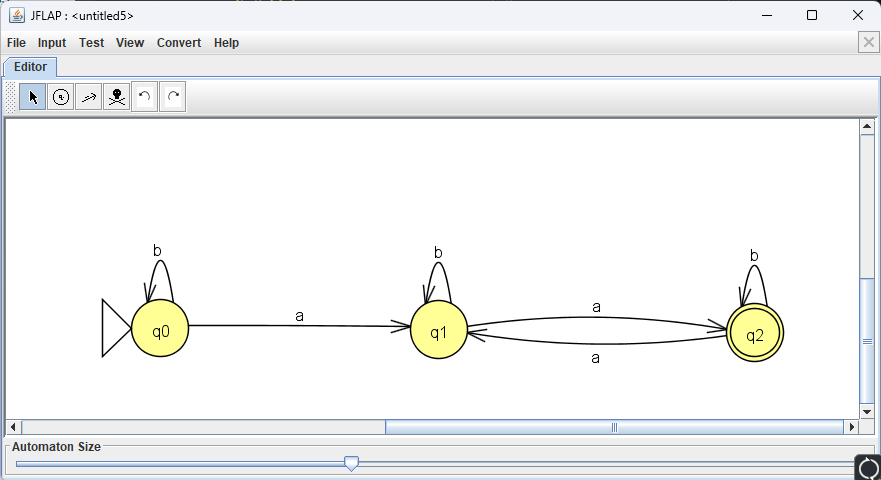
\includegraphics[scale=0.6]{img/DFA_01.png}
  \caption{DFA que reconoce cadenas con número de "a's" par}
\end{figure}

\begin{figure}[H]
  \centering
  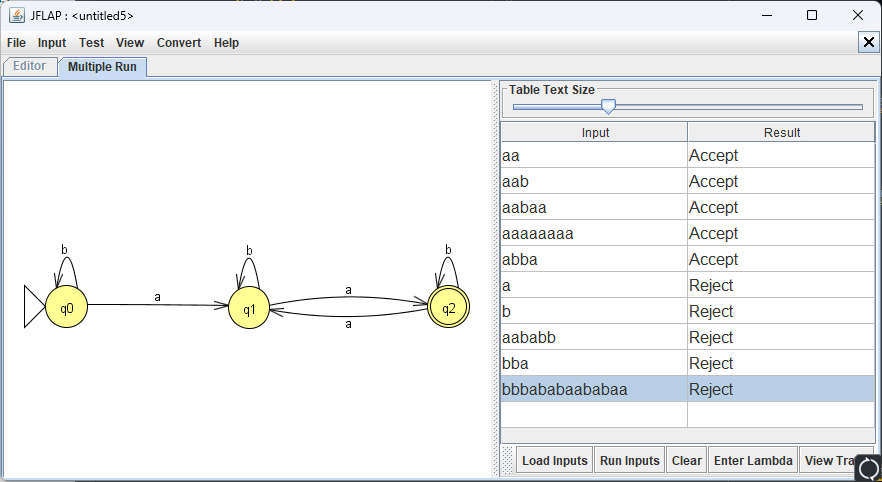
\includegraphics[scale=0.65]{img/DFA_01_test.png}
  \caption{Cadenas de prueba para el DFA}
\end{figure}

\newpage

\section{Diseñar un DFA que reconozca cadenas sobre el alfabeto $\Sigma = \{a, b\}$ con longitud impar.}
\begin{figure}[H]
  \centering
  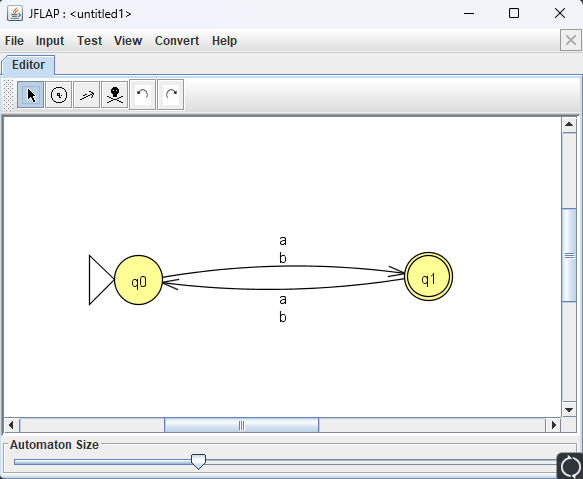
\includegraphics[scale=0.7]{img/DFA_02.png}
  \caption{DFA que reconoce cadenas con longitud impar}
\end{figure}

\begin{figure}[H]
  \centering
  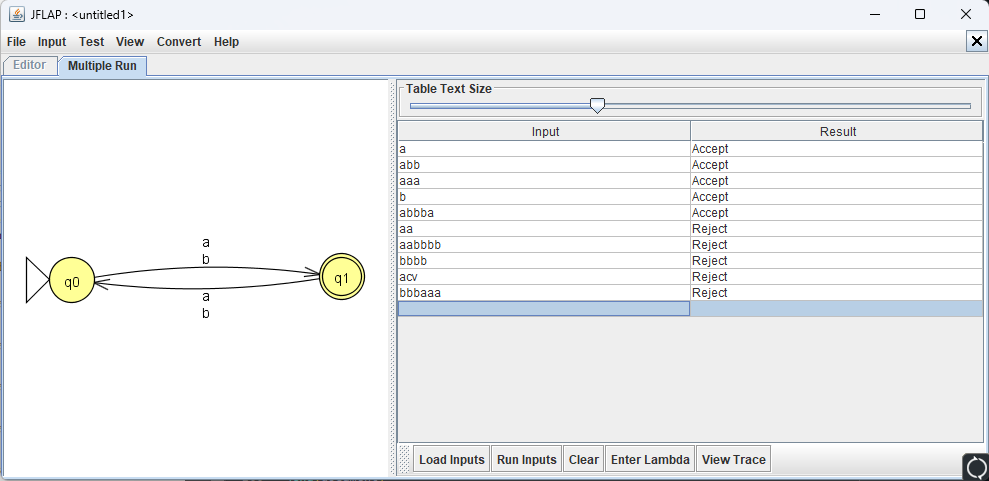
\includegraphics[scale=0.65]{img/DFA_02_test.png}
  \caption{Cadenas de prueba para el DFA}
\end{figure}

\newpage

\section{Diseñar un DFA que reconozca cadenas sobre el alfabeto $\Sigma = \{a, b\}$ con número de “a's” par o longitud impar.}
\begin{figure}[H]
  \centering
  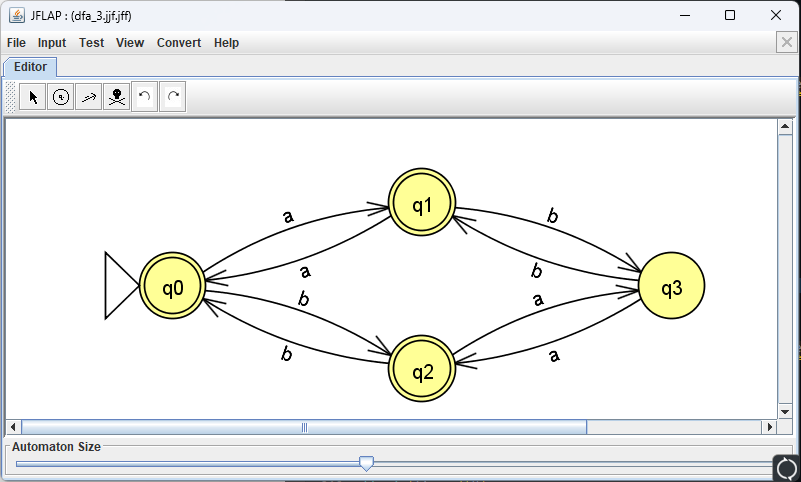
\includegraphics[scale=0.6]{img/DFA_03.png}
  \caption{DFA que reconoce cadenas con número de "a's" par o longitud impar}
\end{figure}

\begin{figure}[H]
  \centering
  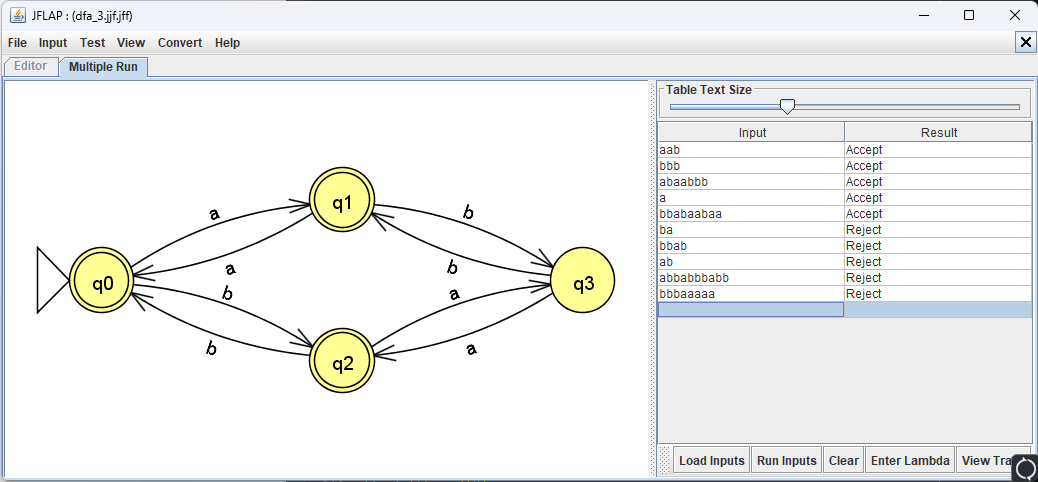
\includegraphics[scale=0.6]{img/DFA_03_test.png}
  \caption{Cadenas de prueba para el DFA}
\end{figure}

\newpage

\section{Diseñar un DFA que reconozca cadenas sobre el alfabeto $\Sigma = \{a, b\}$ con número de “a's” par y longitud impar.}
\begin{figure}[H]
  \centering
  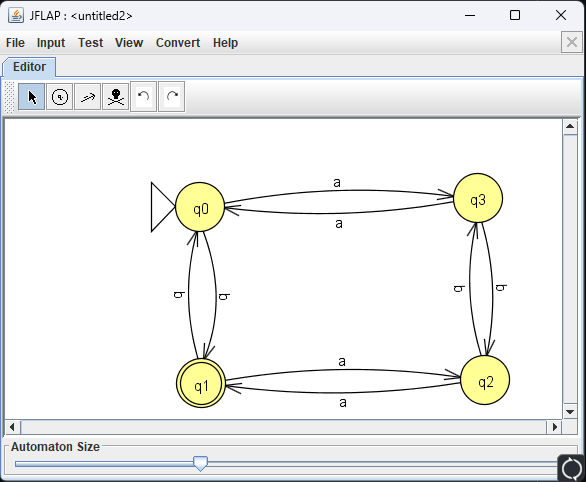
\includegraphics[scale=0.7]{img/DFA_04.png}
  \caption{DFA que reconoce cadenas con número de "a's" par y longitud impar}
\end{figure}

\begin{figure}[H]
  \centering
  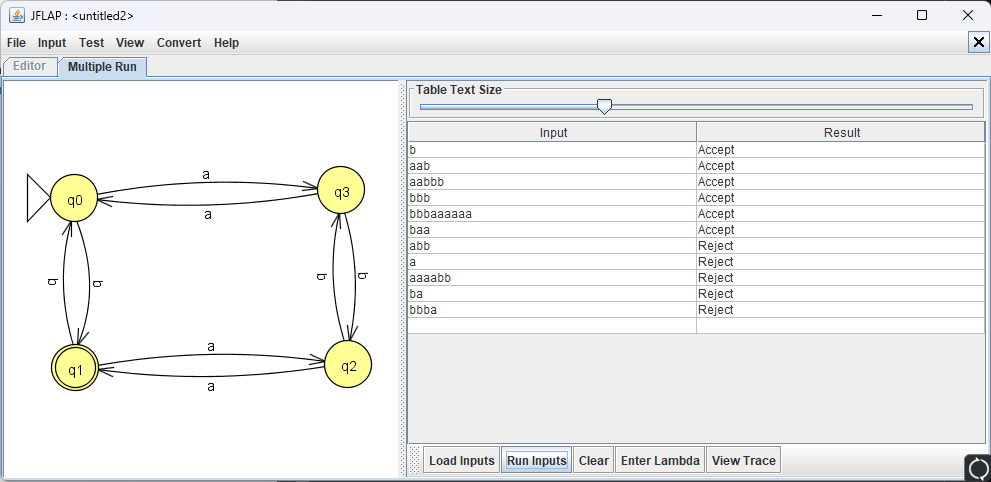
\includegraphics[scale=0.65]{img/DFA_04_test.png}
  \caption{Cadenas de prueba para el DFA}
\end{figure}

\newpage

\section{Diseñar un DFA que reconozca cadenas $w$ sobre el alfabeto $\Sigma = \{0, 1\}$ tales que $2\leq |w| \leq 5$.}
\begin{figure}[H]
  \centering
  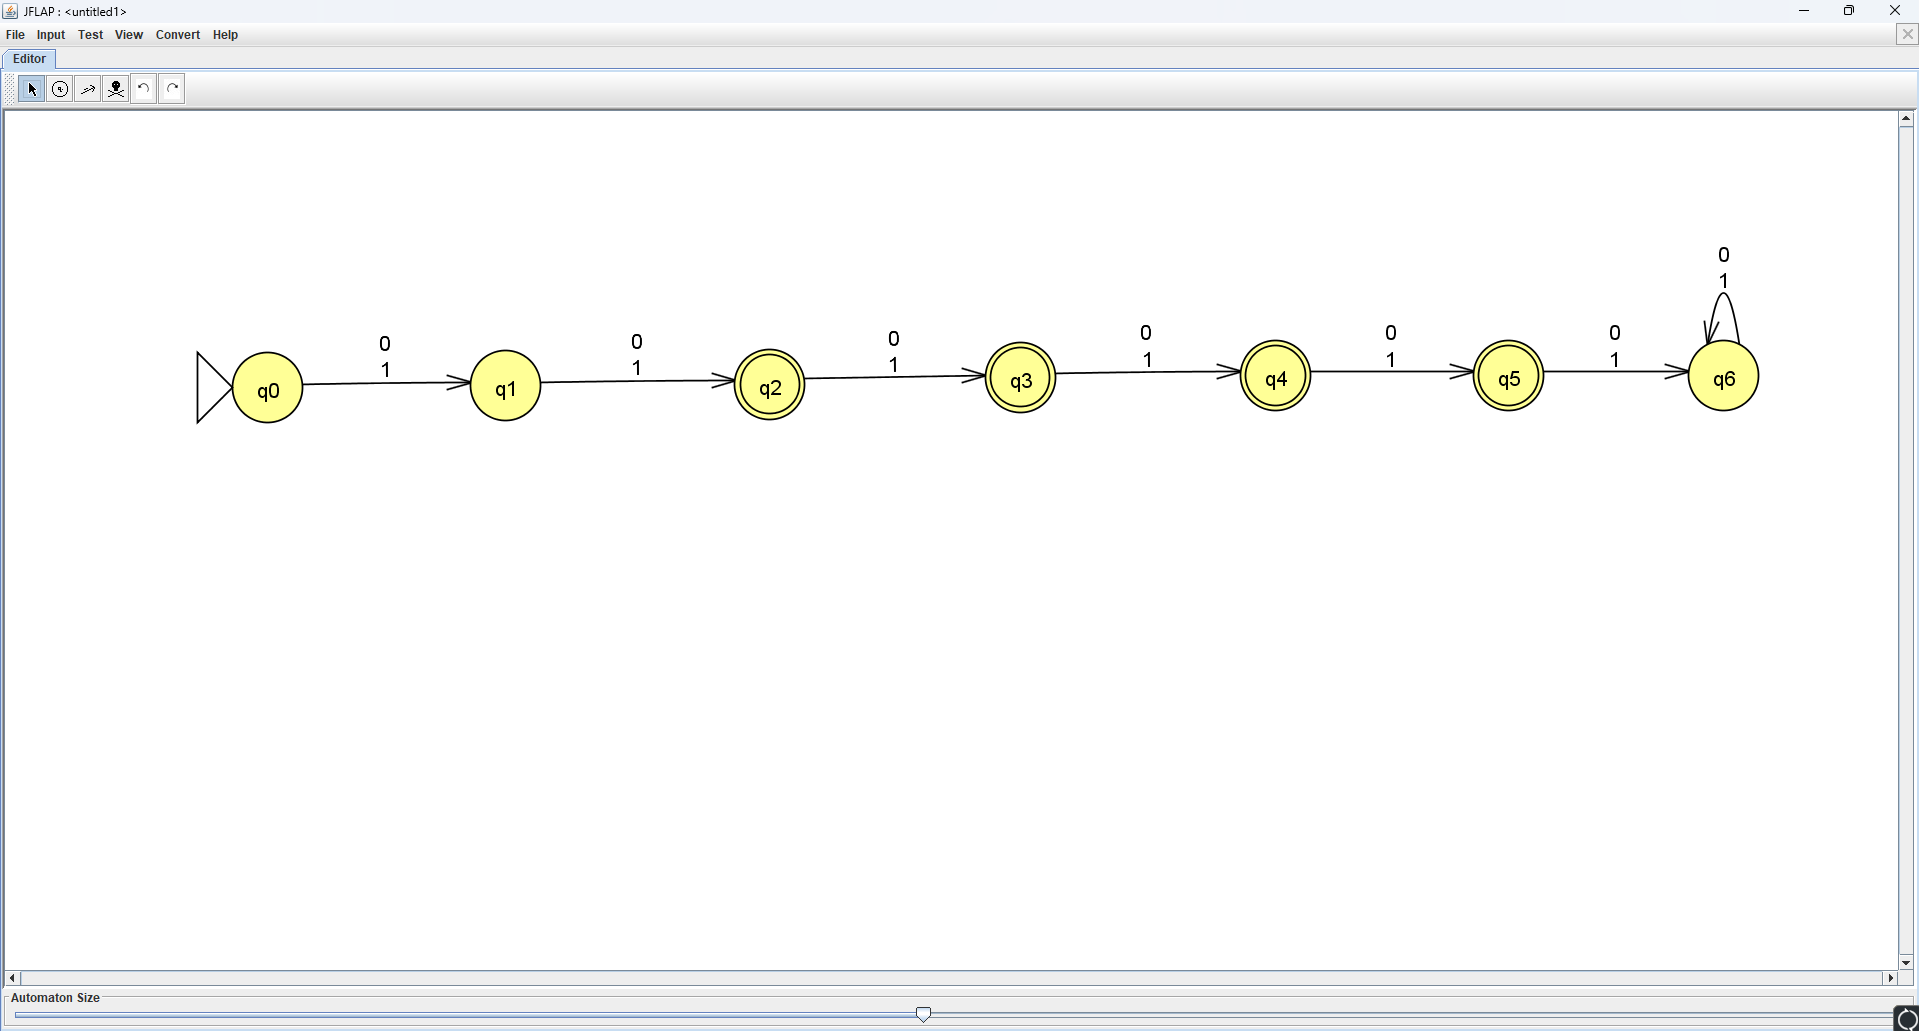
\includegraphics[scale=0.34]{img/DFA_05.png}
  \caption{DFA que reconoce cadenas con longitud entre 2 y 5}
\end{figure}

\begin{figure}[H]
  \centering
  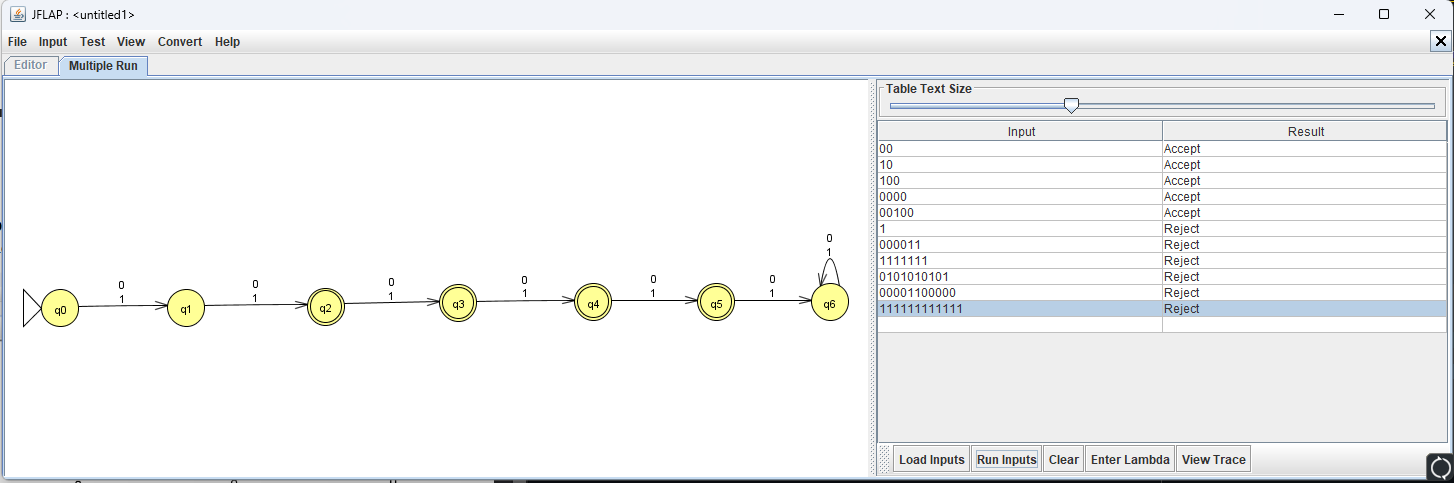
\includegraphics[scale=0.45]{img/DFA_05_test.png}
  \caption{Cadenas de prueba para el DFA}
\end{figure}

\newpage

\section{Diseñar un DFA que reconozca cadenas sobre el alfabeto $\Sigma = \{0, 1\}$ que tengan como minimo dos ceros consecutivos.}
\begin{figure}[H]
  \centering
  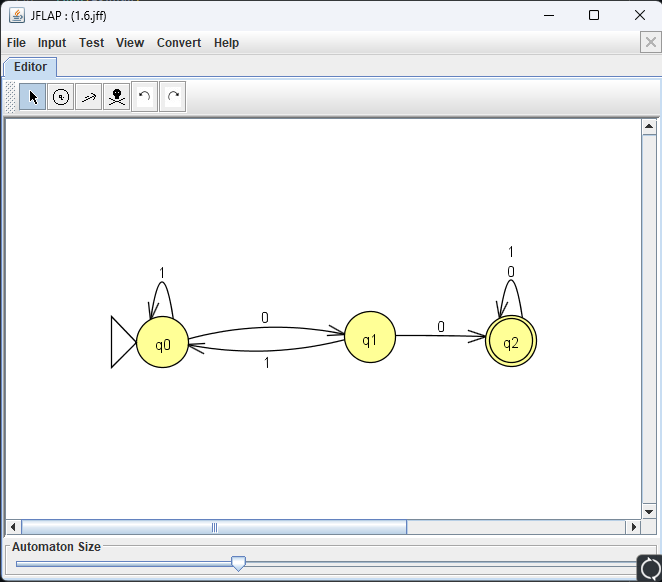
\includegraphics[scale=0.6]{img/DFA_06.png}
  \caption{DFA que reconoce cadenas con al menos dos ceros consecutivos}
\end{figure}

\begin{figure}[H]
  \centering
  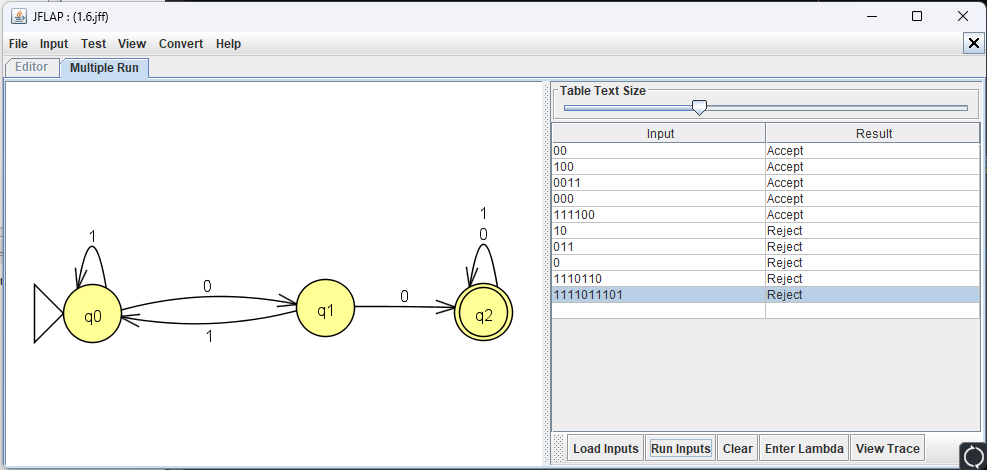
\includegraphics[scale=0.65]{img/DFA_06_test.png}
  \caption{Cadenas de prueba para el DFA}
\end{figure}

\newpage

\section{Diseñar un DFA que reconozca cadenas sobre el alfabeto $\Sigma = \{0, 1\}$ que tengan como máximo dos ceros.}
\begin{figure}[H]
  \centering
  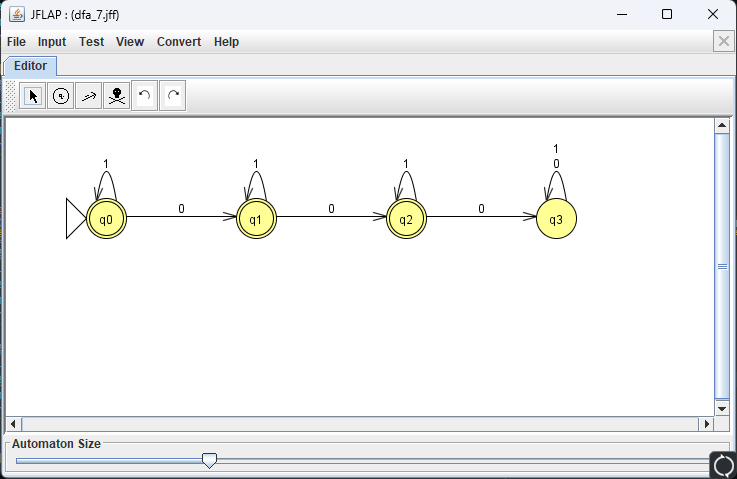
\includegraphics[scale=0.6]{img/DFA_07.png}
  \caption{DFA que reconoce cadenas con como máximo dos ceros}
\end{figure}

\begin{figure}[H]
  \centering
  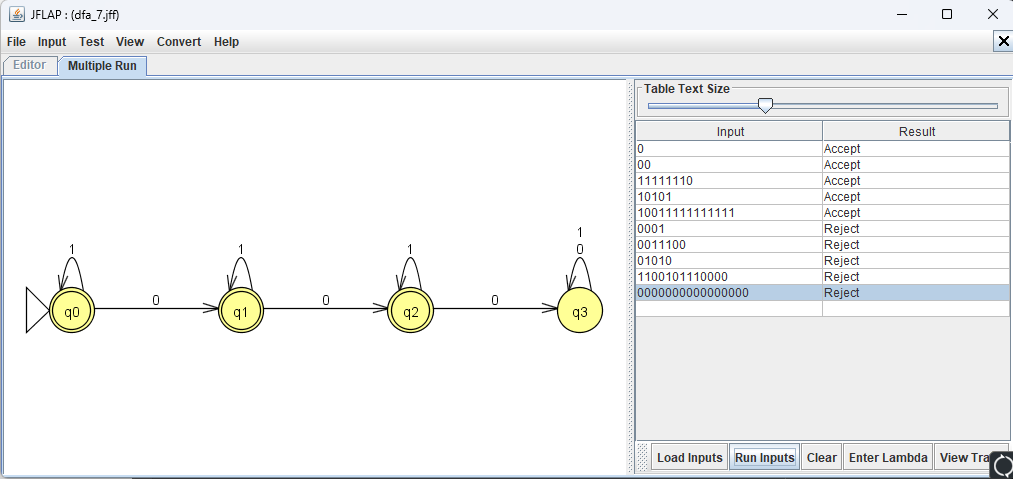
\includegraphics[scale=0.65]{img/DFA_07_test.png}
  \caption{Cadenas de prueba para el DFA}
\end{figure}

\newpage

\section{Diseñar un DFA que reconozca cadenas sobre el alfabeto $\Sigma = \{0, 1\}$ con longitud múltiplo de 3.}
\begin{figure}[H]
  \centering
  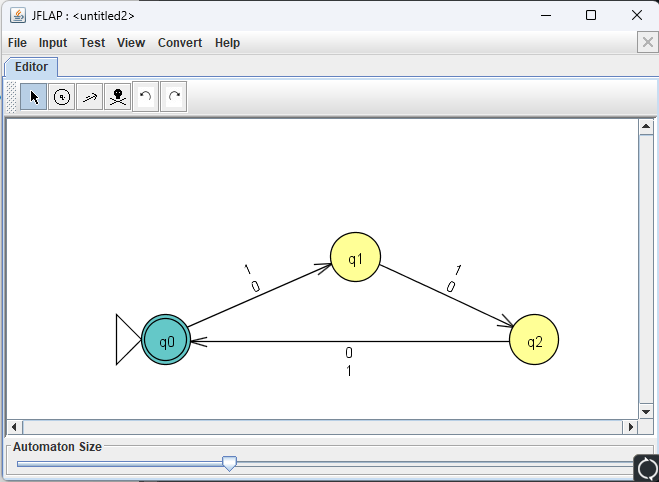
\includegraphics[scale=0.6]{img/DFA_08.png}
  \caption{DFA que reconoce cadenas con longitud múltiplo de 3}
\end{figure}

\begin{figure}[H]
  \centering
  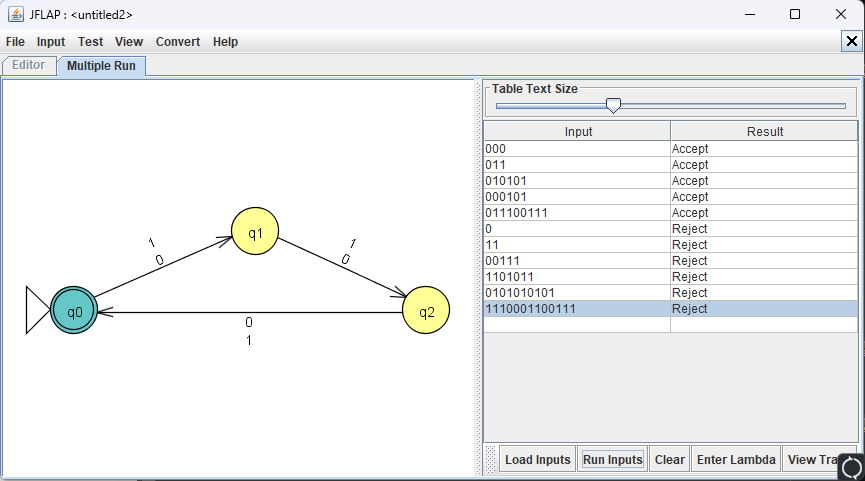
\includegraphics[scale=0.65]{img/DFA_08_test.png}
  \caption{Cadenas de prueba para el DFA}
\end{figure}

\newpage

\section{Diseñar un DFA que reconozca cadenas sobre el alfabeto $\Sigma = \{0, 1\}$ con longitud que no sea múltiplo de 3.}
\begin{figure}[H]
  \centering
  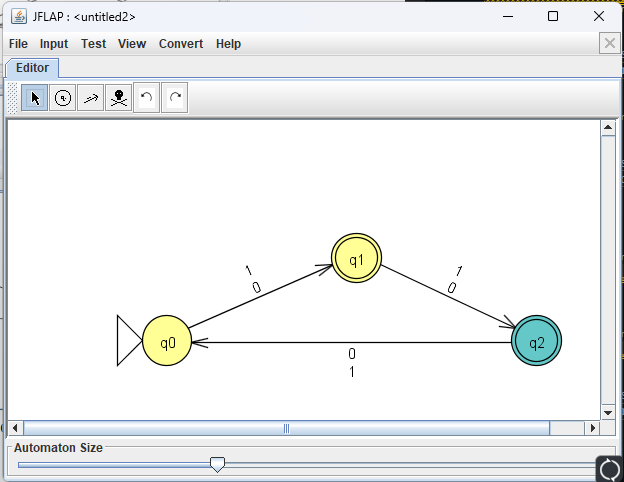
\includegraphics[scale=0.6]{img/DFA_09.png}
  \caption{DFA que reconoce cadenas con longitud que no sea múltiplo de 3}
\end{figure}

\begin{figure}[H]
  \centering
  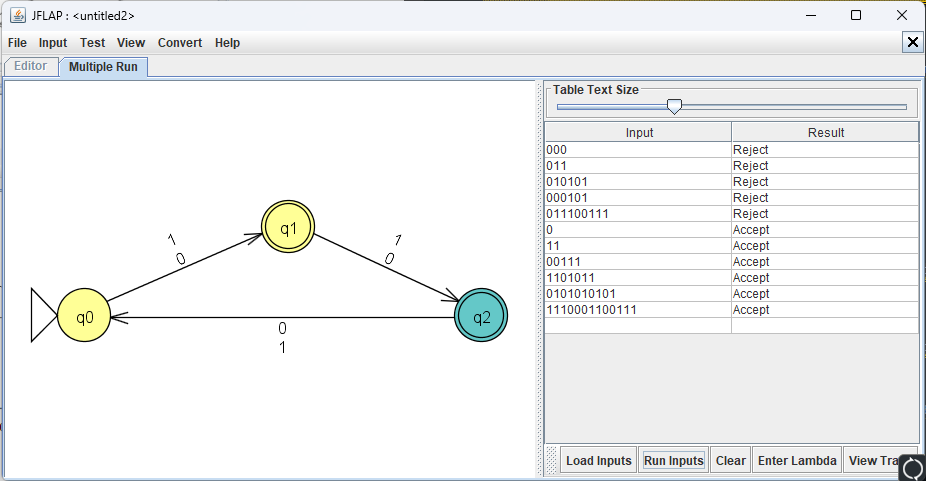
\includegraphics[scale=0.65]{img/DFA_09_test.png}
  \caption{Cadenas de prueba para el DFA}
\end{figure}

\newpage

\section{Diseñar un DFA que reconozca cadenas sobre el alfabeto $\Sigma = \{x, y, z\}$ que no contengan dos símbolos iguales consecutivos.}
\begin{figure}[H]
  \centering
  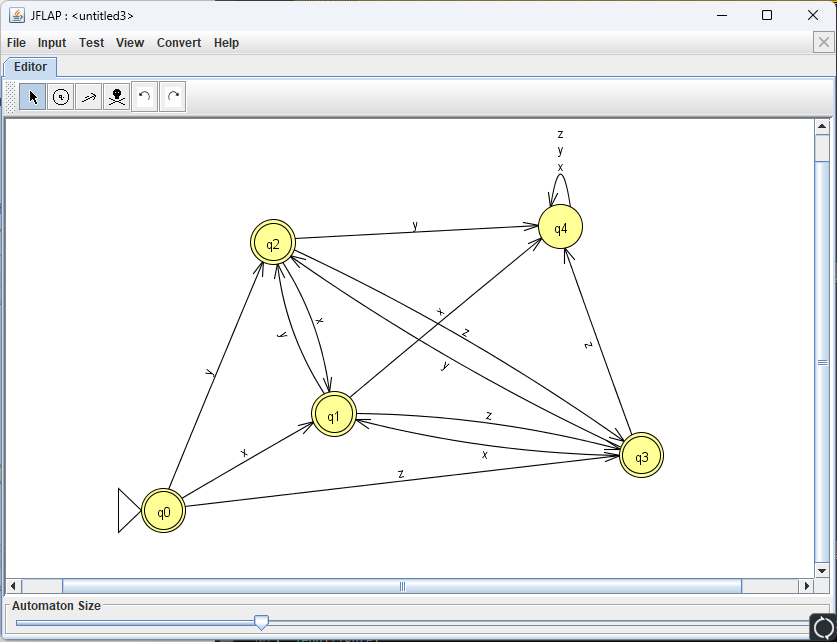
\includegraphics[scale=0.55]{img/DFA_10.png}
  \caption{DFA que reconoce cadenas que no contengan dos símbolos iguales consecutivos}
\end{figure}

\begin{figure}[H]
  \centering
  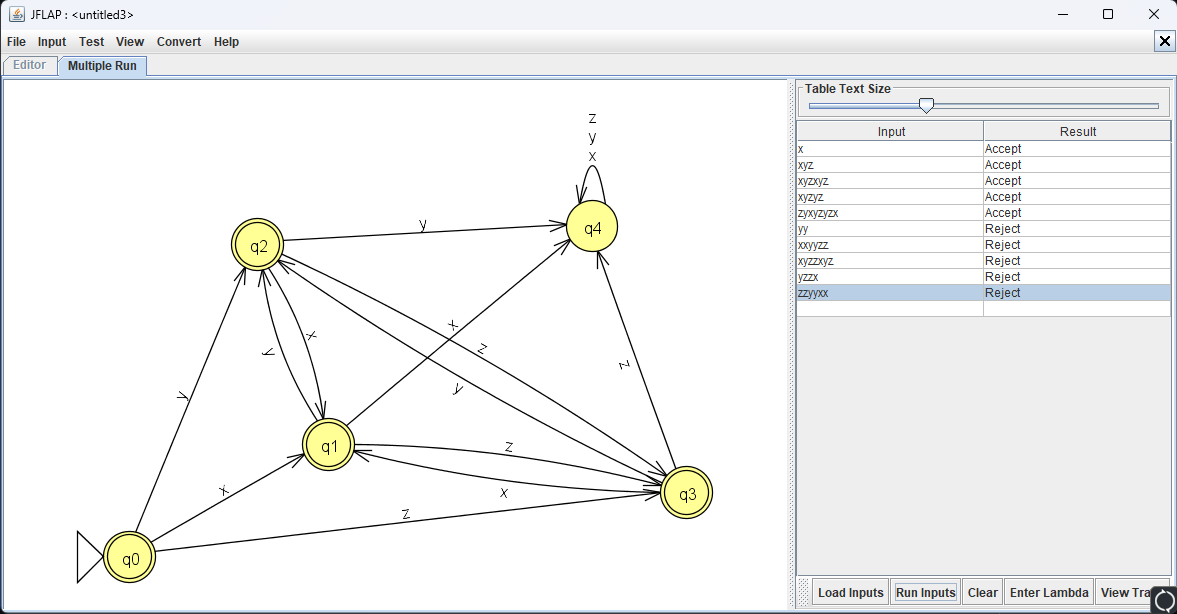
\includegraphics[scale=0.5]{img/DFA_10_test.png}
  \caption{Cadenas de prueba para el DFA}
\end{figure}

\newpage

\chapter{Diseño de NFAs}
\section{Diseñar un NFA que reconozca cadenas sobre el alfabeto $\Sigma = \{a, b\}$ que empiecen por “a”. A partir del NFA diseñado, obtenga un DFA mínimo equivalente.}
\begin{figure}[H]
  \centering
  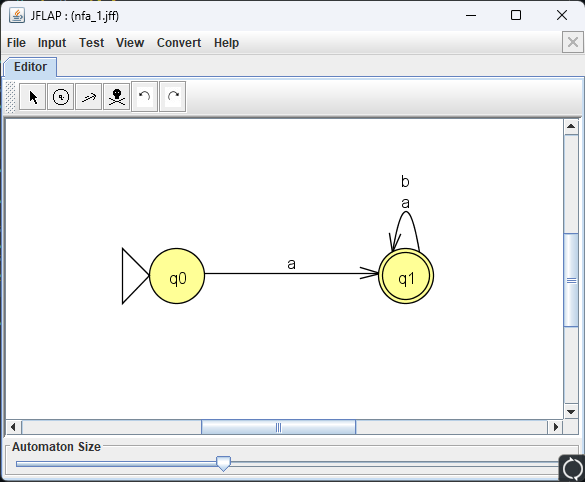
\includegraphics[scale=0.6]{img/NFA_01.png}
  \caption{NFA que reconoce cadenas que empiecen por "a"}
\end{figure}

Algoritmo de construcción de subconjuntos:
\begin{itemize}
  \item $\epsilon$-clausura$(\{q_0\}) = \{q_0\} = A$
  \item $\delta(A, a) = \{q_1\} = B$ 
  \item $\delta(A, b) = \emptyset$
  \item $\delta(B, a) = \{q_1\} = B$
  \item $\delta(B, b) = \{q_1\} = B$
\end{itemize}

\newpage

\section{Diseñar un NFA que reconozca cadenas sobre el alfabeto $\Sigma = \{a, b\}$ que terminen en “bb”. A partir del NFA diseñado, obtenga un DFA mínimo equivalente.}
\begin{figure}[H]
  \centering
  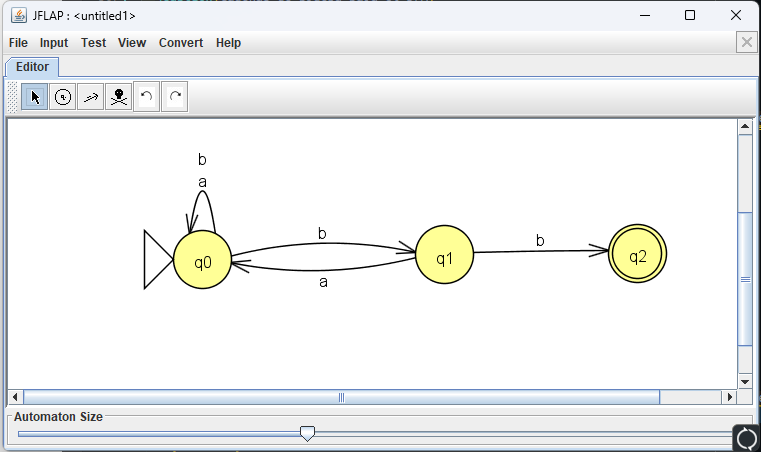
\includegraphics[scale=0.6]{img/NFA_02.png}
  \caption{NFA que reconoce cadenas que terminen en "bb"}
\end{figure}

\begin{figure}[H]
  \centering
  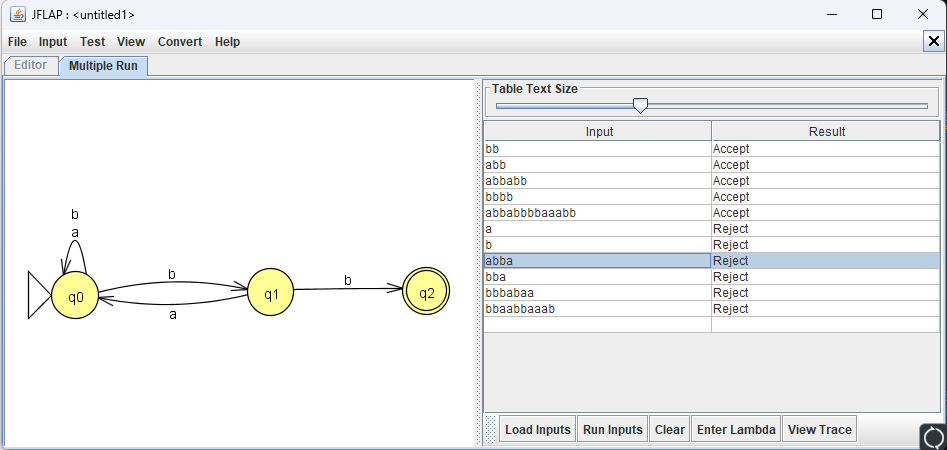
\includegraphics[scale=0.6]{img/NFA_02_test.png}
  \caption{Cadenas de prueba para el NFA}
\end{figure}

\newpage

Algoritmo de construcción de subconjuntos:
\begin{multicols}{2}
  \begin{itemize}
    \item $\epsilon$-clausura$(\{q_0\}) = \{q_0\} = A$
    \item $\delta(A, a) = \{q_0\} = A$
    \item $\delta(A, b) = \{q_0, q_1\} = B$
    \item $\delta(B, a) = \{q_0\} = A$
  \end{itemize}

  \columnbreak

  \begin{itemize}
    \item $\delta(B, b) = \{q_0, q_1, q_2\} = C$
    \item $\delta(C, a) = \{q_0\} = A$
    \item $\delta(C, b) = \{q_0, q_1, q_2\} = C$ 
  \end{itemize}
\end{multicols}

\begin{figure}[H]
  \centering
  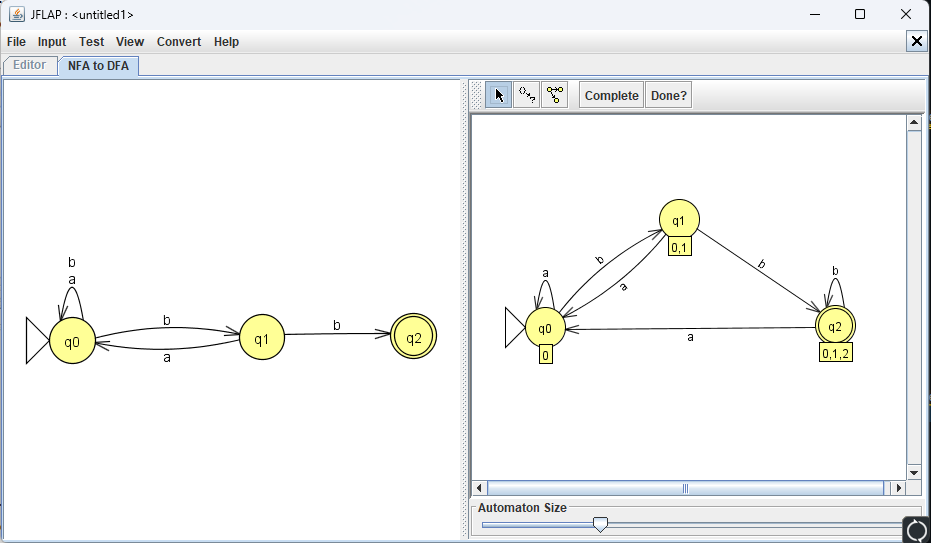
\includegraphics[scale=0.45]{img/NFA_to_DFA_02.png}
  \caption{DFA equivalente al NFA}
\end{figure}

Algoritmo de minimización de DFA:
\begin{itemize}
  \item $\{C\} \{A, B\}$
  \item $\{C\} \{A\} \{B\}$
\end{itemize}

El DFA ya está minimizado.

\begin{figure}[H]
  \centering
  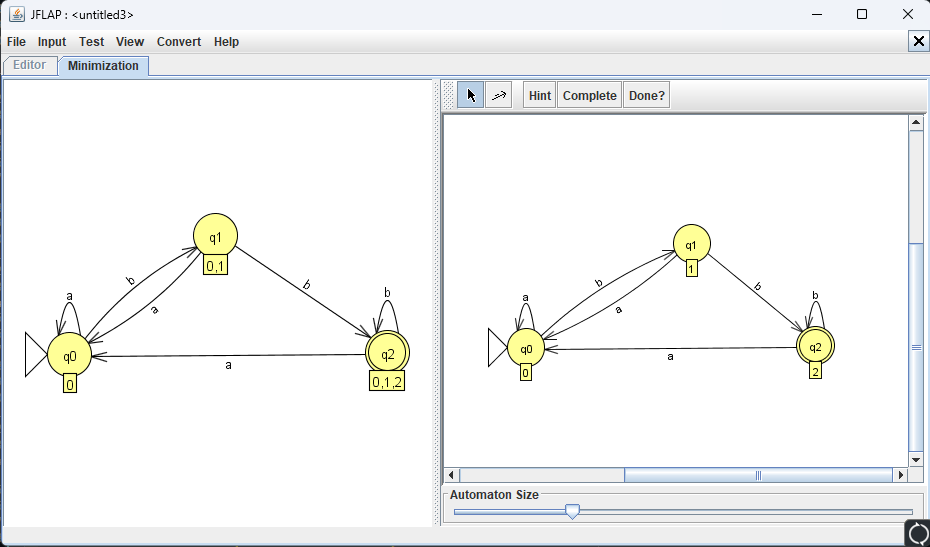
\includegraphics[scale=0.4]{img/DFA_to_DFA_minimized_02.png}
  \caption{DFA mínimo equivalente al NFA}
\end{figure}

\newpage

\section{Diseñar un NFA que reconozca cadenas sobre el alfabeto $\Sigma = \{a, b\}$ que empiecen por “a” o terminen en “bb”. A partir del NFA diseñado, obtenga un DFA mínimo equivalente.}

\newpage

\section{Diseñar un NFA que reconozca cadenas sobre el alfabeto $\Sigma = \{a, b\}$ que empiecen por “a” y terminen en “bb”. A partir del NFA diseñado, obtenga un DFA mínimo equivalente.}
\begin{figure}[H]
  \centering
  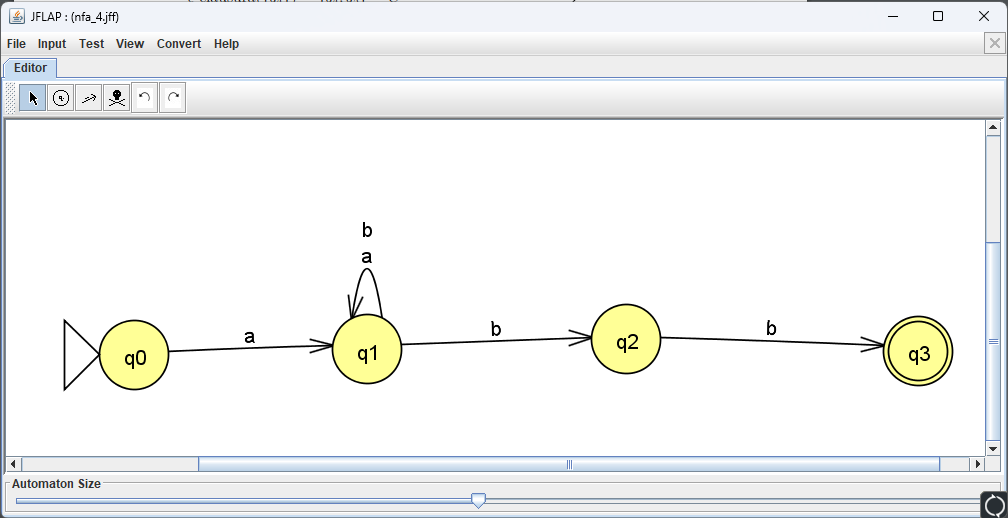
\includegraphics[scale=0.6]{img/NFA_04.png}
  \caption{NFA que reconoce cadenas que empiecen por "a" y terminen en "bb"}
\end{figure}

\begin{figure}[H]
  \centering
  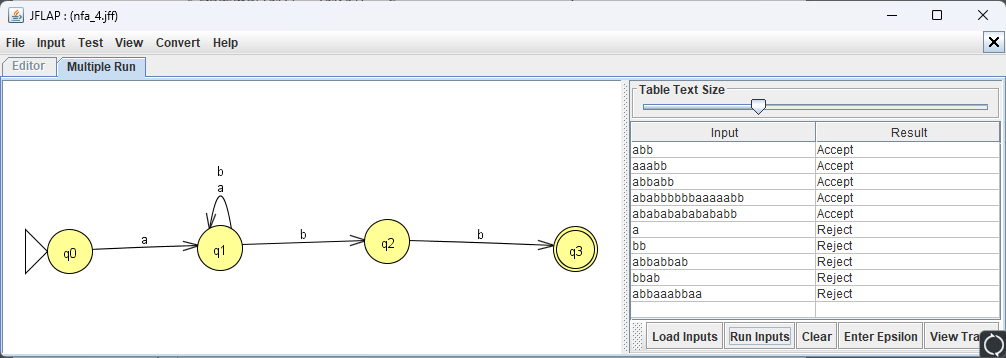
\includegraphics[scale=0.55]{img/NFA_04_test.png}
  \caption{Cadenas de prueba para el NFA}
\end{figure}

\newpage

Algoritmo de construcción de subconjuntos:
\begin{multicols}{2}
  \begin{itemize}
    \item $\epsilon$-clausura$(\{q_0\}) = \{q_0\} = A$
    \item $\delta(A, a) = \{q_1\} = B$
    \item $\delta(A, b) = \emptyset$
    \item $\delta(B, a) = \{q_1\} = B$
    \item $\delta(B, b) = \{q_1, q_2\} = C$
  \end{itemize}

  \columnbreak

  \begin{itemize}
    \item $\delta(C, a) = \{q_1\} = B$
    \item $\delta(C, b) = \{q_1, q_2, q_3\} = D$
    \item $\delta(D, a) = \{q_1\} = B$
    \item $\delta(D, b) = \{q_1, q_2, q_3\} = D$
  \end{itemize}  
\end{multicols}

\begin{figure}[H]
  \centering
  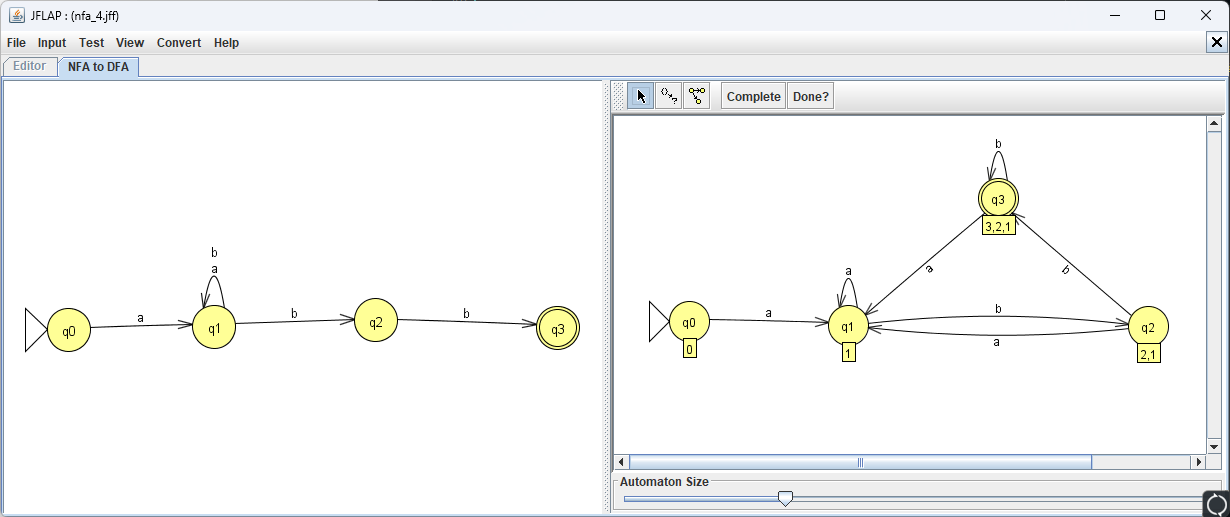
\includegraphics[scale=0.4]{img/NFA_to_DFA_04.png}
  \caption{DFA equivalente al NFA}
\end{figure}

Algoritmo de minimización de DFA:
\begin{itemize}
  \item $\{D\} \{A, B, C\}$
  \item $\{D\} \{A\} \{B, C\}$
  \item $\{D\} \{A\} \{B\} \{C\}$
\end{itemize}

El DFA ya está minimizado.

\begin{figure}[H]
  \centering
  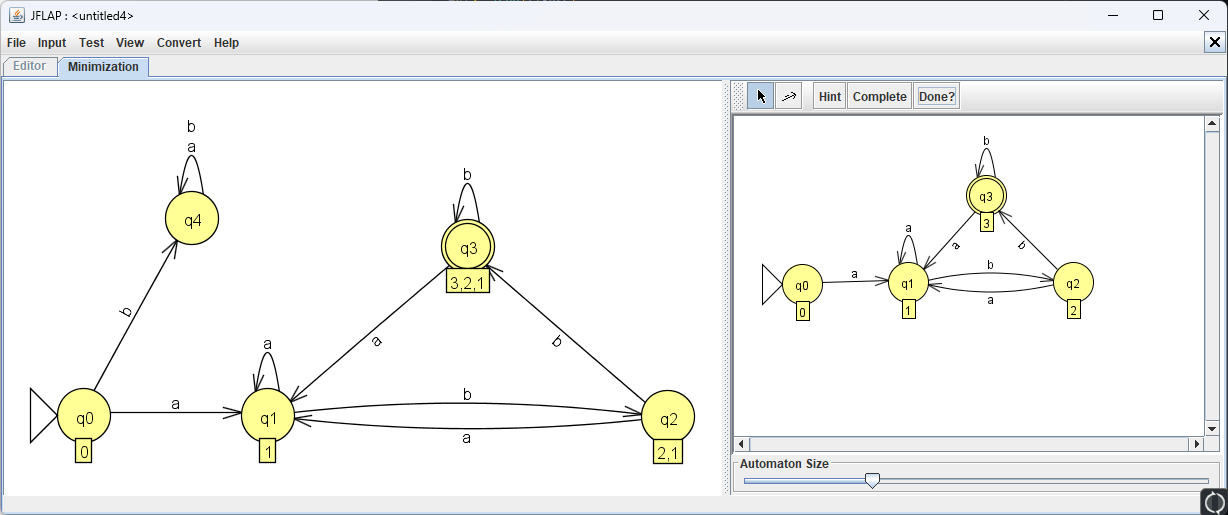
\includegraphics[scale=0.4]{img/DFA_to_DFA_minimized_04.png}
  \caption{DFA mínimo equivalente al NFA}
\end{figure}

\newpage

\section{Diseñar un NFA que reconozca cadenas sobre el alfabeto $\Sigma = \{a, b\}$ con número de “a's” par o longitud impar. A partir del NFA diseñado, obtenga un DFA mínimo equivalente.}

\newpage

\section{Diseñar un NFA que reconozca cadenas sobre el alfabeto $\Sigma = \{x, y, z\}$ que contenga al menos dos símbolos iguales consecutivos. A partir del NFA diseñado, obtenga un DFA mínimo equivalente.}
\begin{figure}[H]
  \centering
  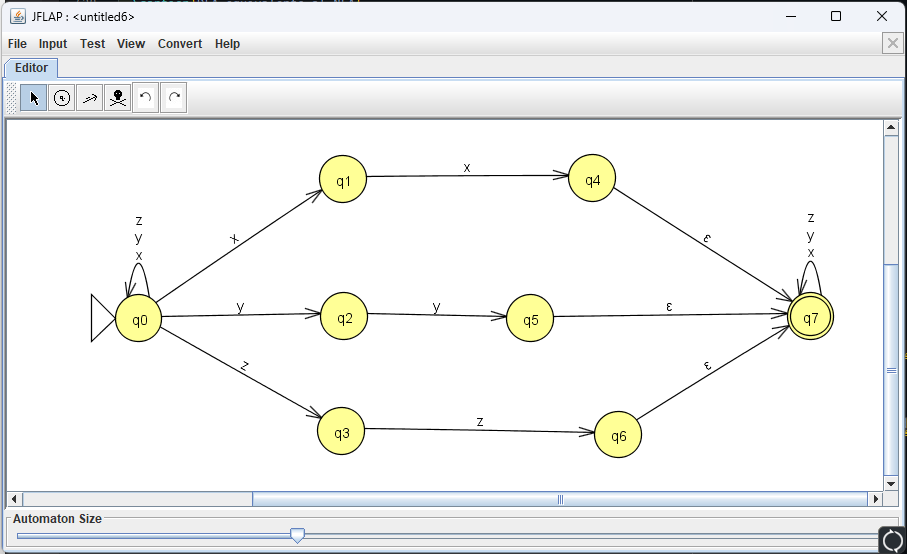
\includegraphics[scale=0.55]{img/NFA_06.png}
  \caption{NFA que reconoce cadenas con al menos dos símbolos iguales consecutivos}
\end{figure}

\begin{figure}[H]
  \centering
  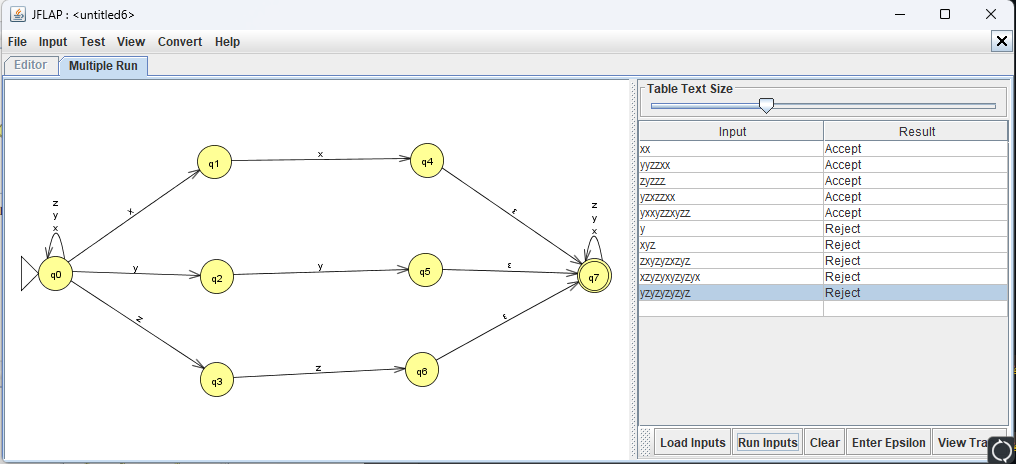
\includegraphics[scale=0.5]{img/NFA_06_test.png}
  \caption{Cadenas de prueba para el NFA}
\end{figure}

\newpage

Algoritmo de construcción de subconjuntos:
\begin{multicols}{2}
  \begin{itemize}
    \item $\epsilon$-clausura$(\{q_0\}) = \{q_0\} = A$
    \item $\delta(A, x) = \{q_0, q_1\}$ = B
    \item $\delta(A, y) = \{q_0, q_2\}$ = C
    \item $\delta(A, z) = \{q_0, q_3\}$ = D
    \item $\delta(B, x) = \{q_0, q_1, q_4\}$ = E
    \item $\delta(B, y) = \{q_0, q_2\}$ = C
    \item $\delta(B, z) = \{q_0, q_3\}$ = D
    \item $\delta(C, x) = \{q_0, q_1\}$ = B
    \item $\delta(C, y) = \{q_0, q_2, q_4\}$ = F
    \item $\delta(C, z) = \{q_0, q_3\}$ = D
    \item $\delta(D, x) = \{q_0, q_1\}$ = B
  \end{itemize}
  
  \columnbreak

  \begin{itemize}
    \item $\delta(D, y) = \{q_0, q_2\}$ = C
    \item $\delta(D, z) = \{q_0, q_3, q_4\}$ = G
    \item $\delta(E, x) = \{q_0, q_1, q_4\}$ = E
    \item $\delta(E, y) = \{q_0, q_2, q_4\}$ = F
    \item $\delta(E, z) = \{q_0, q_3, q_4\}$ = G
    \item $\delta(F, x) = \{q_0, q_1, q_4\}$ = E
    \item $\delta(F, y) = \{q_0, q_2, q_4\}$ = F
    \item $\delta(F, z) = \{q_0, q_3, q_4\}$ = G
    \item $\delta(G, x) = \{q_0, q_1, q_4\}$ = E
    \item $\delta(G, y) = \{q_0, q_2, q_4\}$ = F
    \item $\delta(G, z) = \{q_0, q_3, q_4\}$ = G
  \end{itemize}
\end{multicols}

\begin{figure}[H]
  \centering
  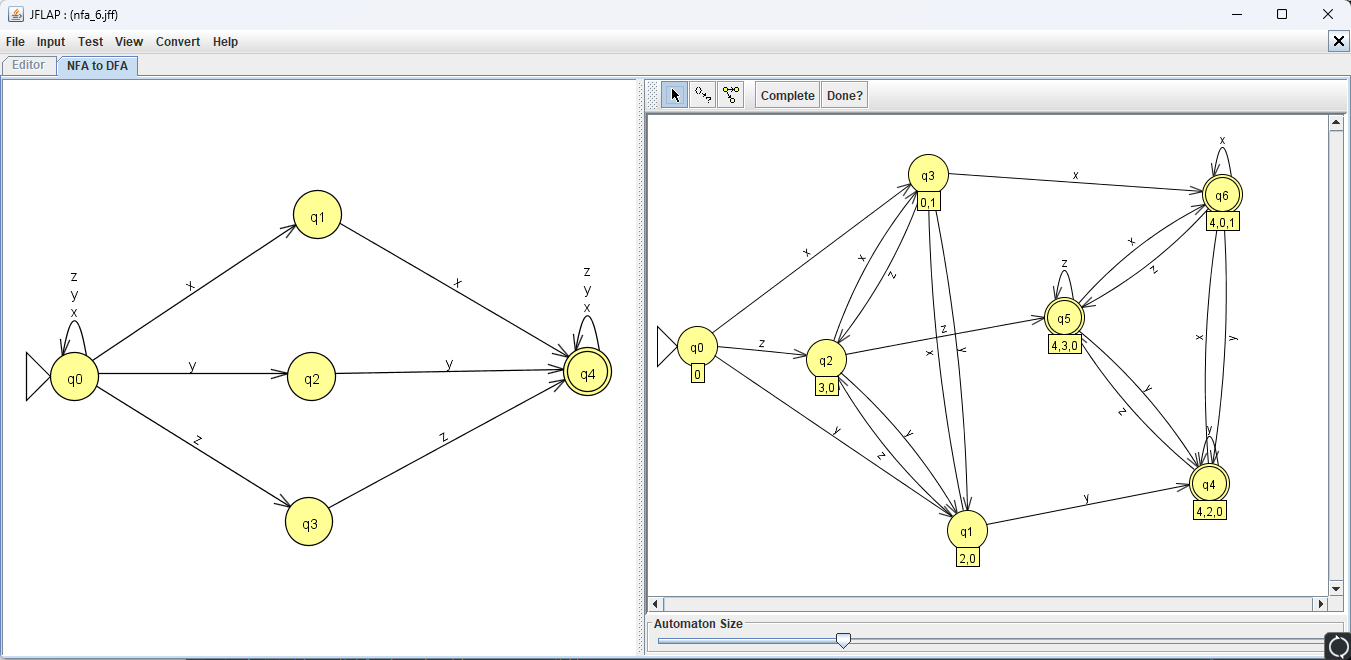
\includegraphics[scale=0.45]{img/NFA_to_DFA_06.png}
  \caption{DFA equivalente al NFA}
\end{figure}

Algoritmo de minimización de DFA:
\begin{itemize}
  \item $\{E, F, G\} \{A, B, C, D\}$
  \item $\{E, F, G\} \{B\} \{A, C, D\}$
  \item $\{E, F, G\} \{B\} \{C\} \{A, D\}$
  \item $\{E, F, G\} \{B\} \{C\} \{D\} \{A\}$
\end{itemize}

El DFA minimizado es el siguiente:
\begin{figure}[H]
  \centering
  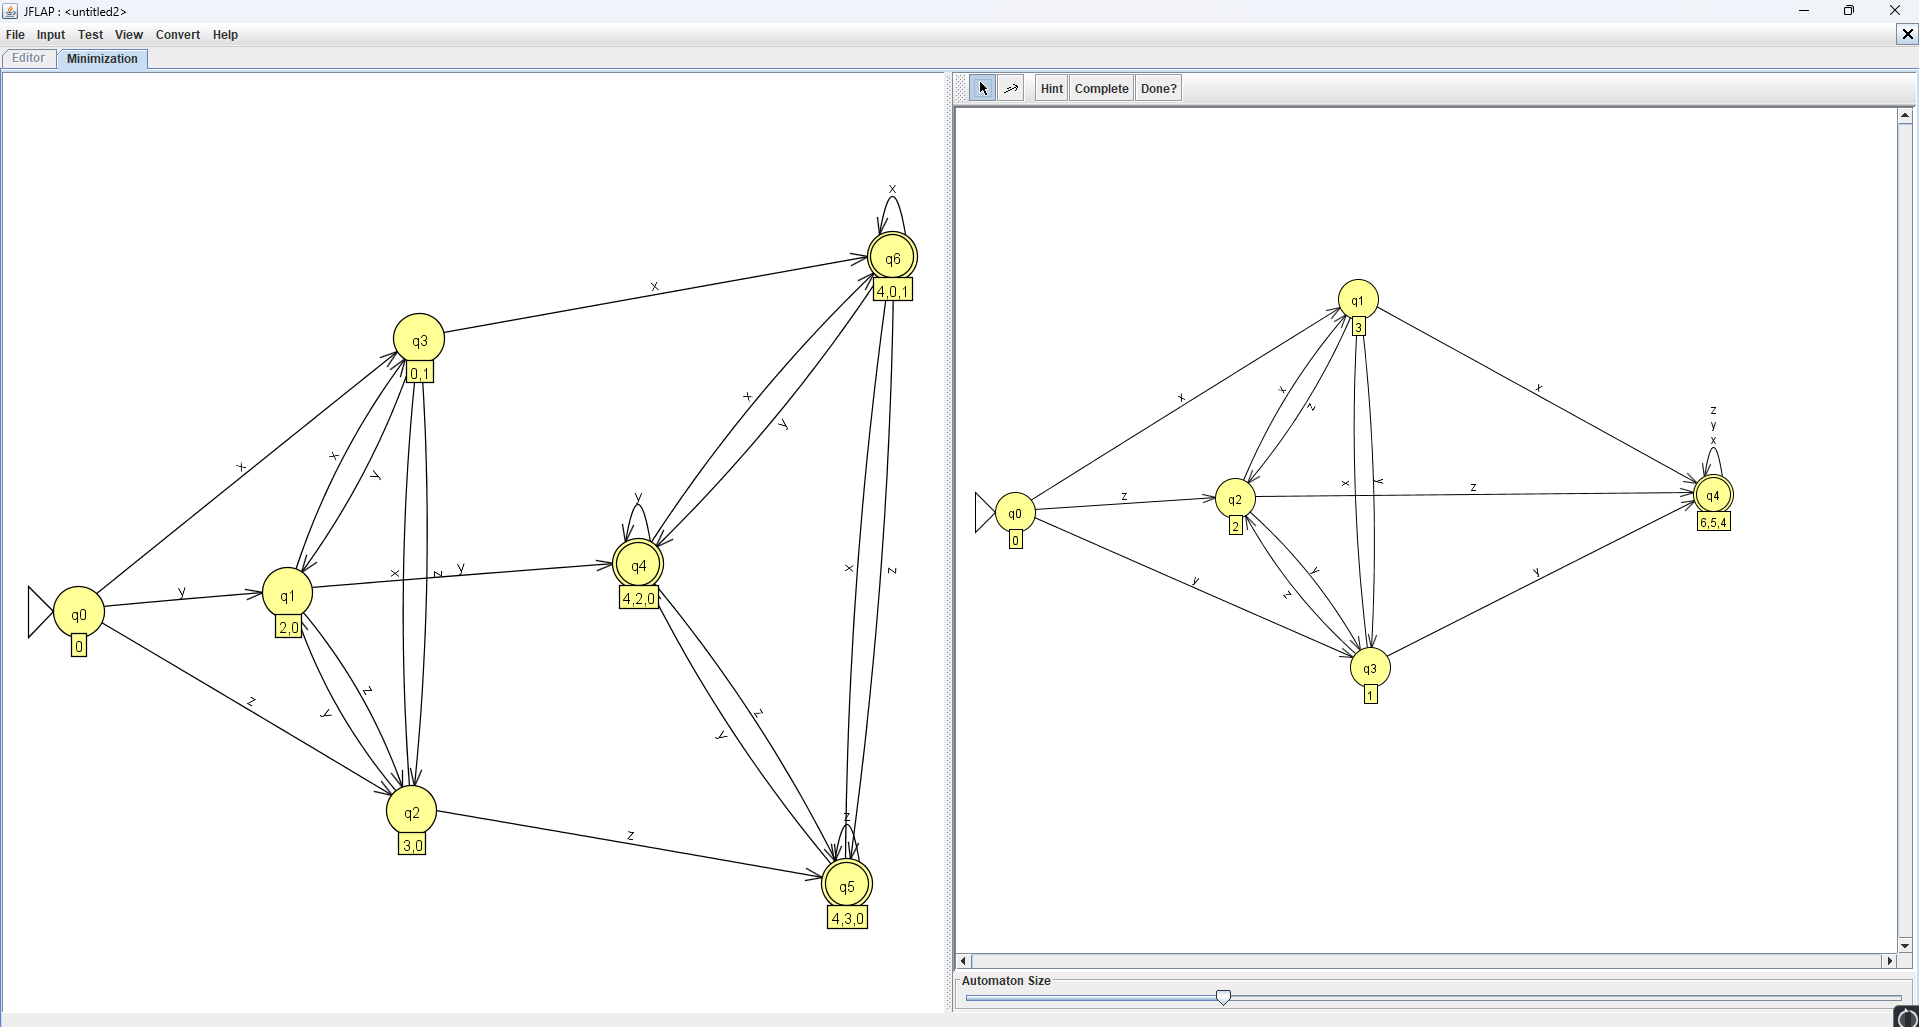
\includegraphics[scale=0.3]{img/DFA_to_DFA_minimized_06.png}
  \caption{DFA mínimo equivalente al NFA}
\end{figure}

\newpage

\section{Diseñar un NFA que reconozca cadenas $w$ sobre el alfabeto $\Sigma = \{x, y, z\}$ con $|w| \geq 2$, tales que $w$ empieza y termina por el mismo símbolo. A partir del NFA diseñado, obtenga un DFA mínimo equivalente.}
\begin{figure}[H]
  \centering
  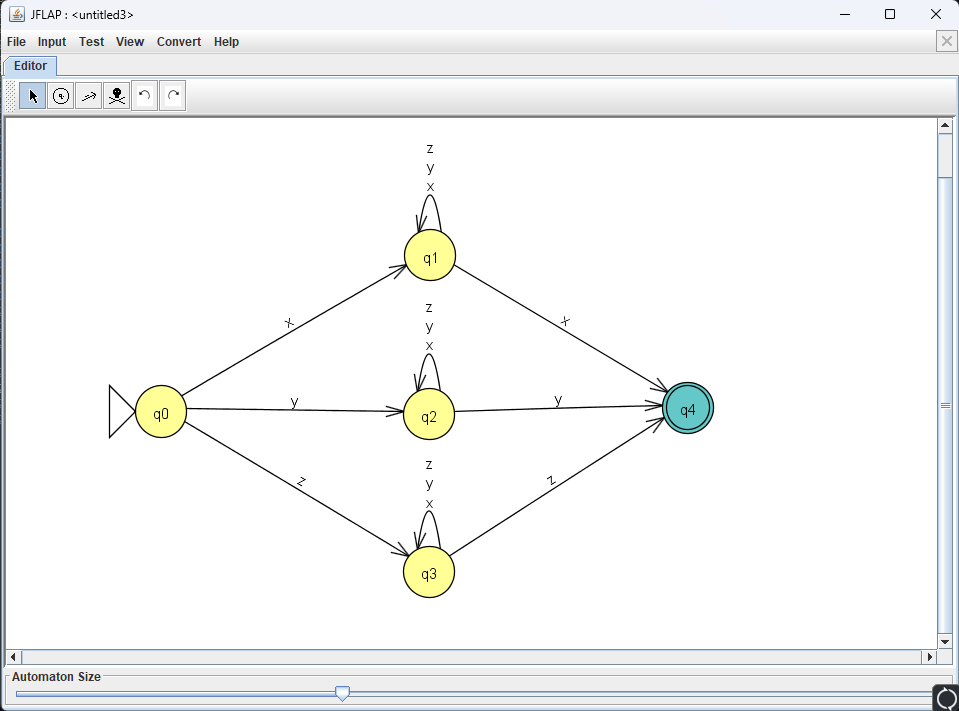
\includegraphics[scale=0.4]{img/NFA_07.png}
  \caption{NFA que reconoce cadenas que empiezan y terminan por el mismo símbolo}
\end{figure}

\begin{figure}[H]
  \centering
  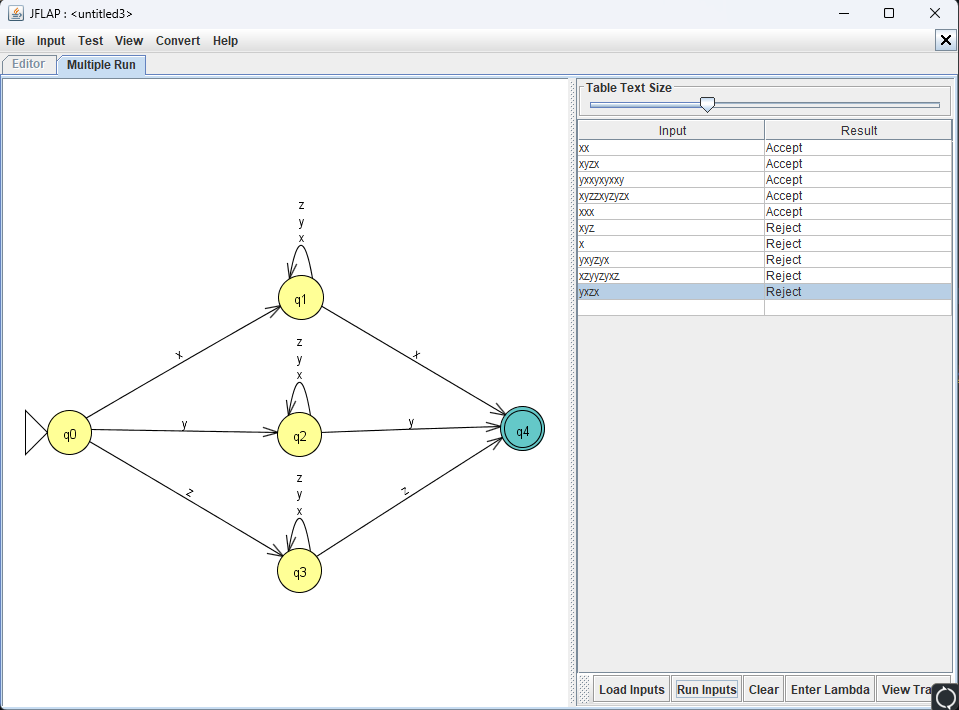
\includegraphics[scale=0.45]{img/NFA_07_test.png}
  \caption{Cadenas de prueba para el NFA}
\end{figure}

\newpage

Algoritmo de construcción de subconjuntos:
\begin{multicols}{2}
  \begin{itemize}
    \item $\epsilon$-clausura$(\{q_0\}) = \{q_0\} = A$
    \item $\delta(A, x) = \{q_1\}$ = B
    \item $\delta(A, y) = \{q_2\}$ = C
    \item $\delta(A, z) = \{q_3\}$ = D
    \item $\delta(B, x) = \{q_1, q_4\}$ = E
    \item $\delta(B, y) = \{q_1\}$ = B
    \item $\delta(B, z) = \{q_1\}$ = B
    \item $\delta(C, x) = \{q_2\}$ = C
    \item $\delta(C, y) = \{q_2, q_4\}$ = F
    \item $\delta(C, z) = \{q_2\}$ = C
    \item $\delta(D, x) = \{q_3\}$ = D
  \end{itemize}

  \columnbreak

  \begin{itemize}
    \item $\delta(D, y) = \{q_3\}$ = D
    \item $\delta(D, z) = \{q_3, q_4\}$ = G
    \item $\delta(E, x) = \{q_1, q_4\}$ = E
    \item $\delta(E, y) = \{q_1\}$ = B
    \item $\delta(E, z) = \{q_1\}$ = B
    \item $\delta(F, x) = \{q_2\}$ = C
    \item $\delta(F, y) = \{q_2, q_4\}$ = F
    \item $\delta(F, z) = \{q_2\}$ = C
    \item $\delta(G, x) = \{q_3\}$ = D
    \item $\delta(G, y) = \{q_3\}$ = D
    \item $\delta(G, z) = \{q_3, q_4\}$ = G
  \end{itemize}
\end{multicols}

\begin{figure}[H]
  \centering
  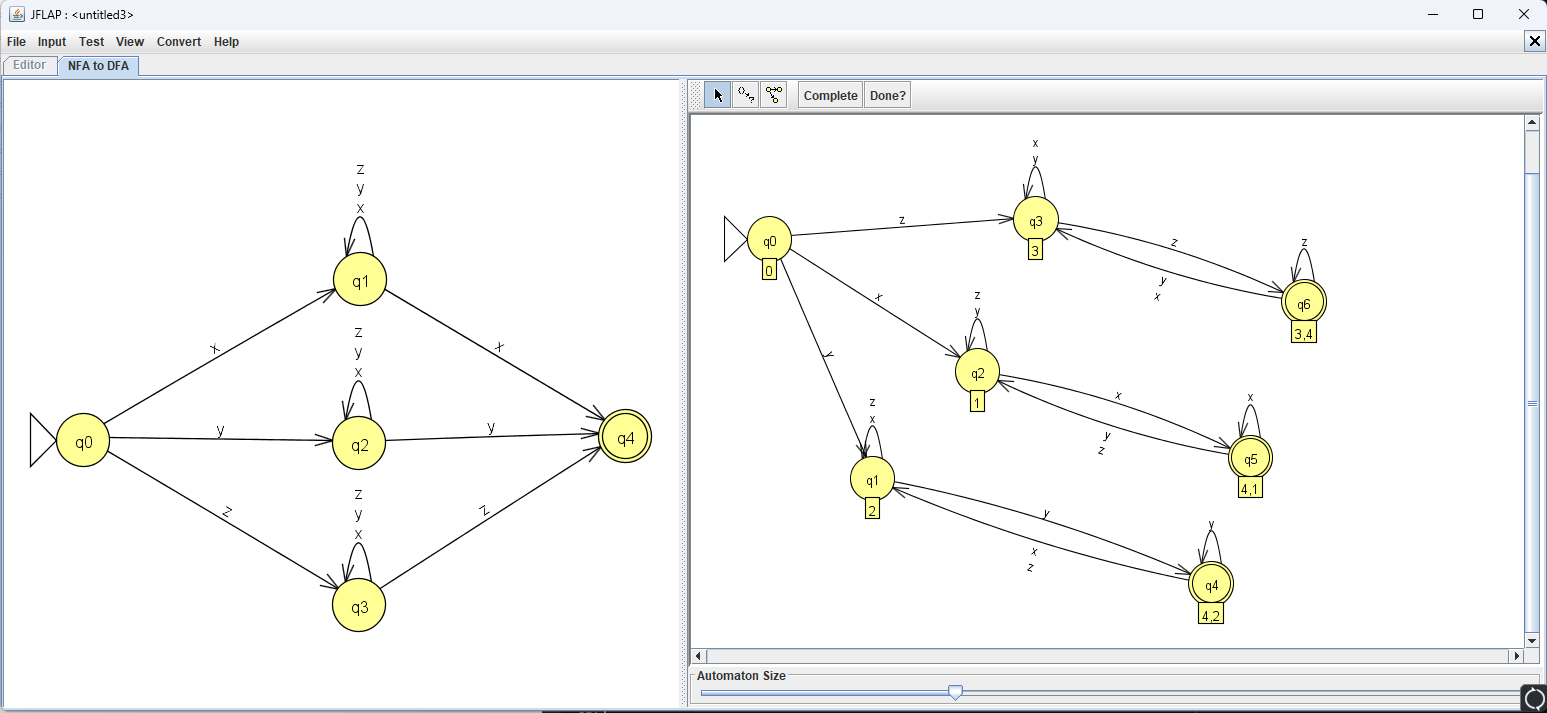
\includegraphics[scale=0.4]{img/NFA_to_DFA_07.png}
  \caption{DFA equivalente al NFA}
\end{figure}

\newpage

Algoritmo de minimización de DFA:
\begin{itemize}
  \item $\{E, F, G\} \{A, B, C, D\}$
  \item $\{E, F, G\} \{B\} \{A, C, D\}$
  \item $\{E, F, G\} \{B\} \{C\} \{A, D\}$
  \item $\{E, F, G\} \{B\} \{C\} \{D\} \{A\}$
  \item $\{E, G\} \{F\} \{B\} \{C\} \{D\} \{A\}$
  \item $\{E\} \{G\} \{F\} \{B\} \{C\} \{D\} \{A\}$
\end{itemize}

El DFA ya está minimizado.
\begin{figure}[H]
  \centering
  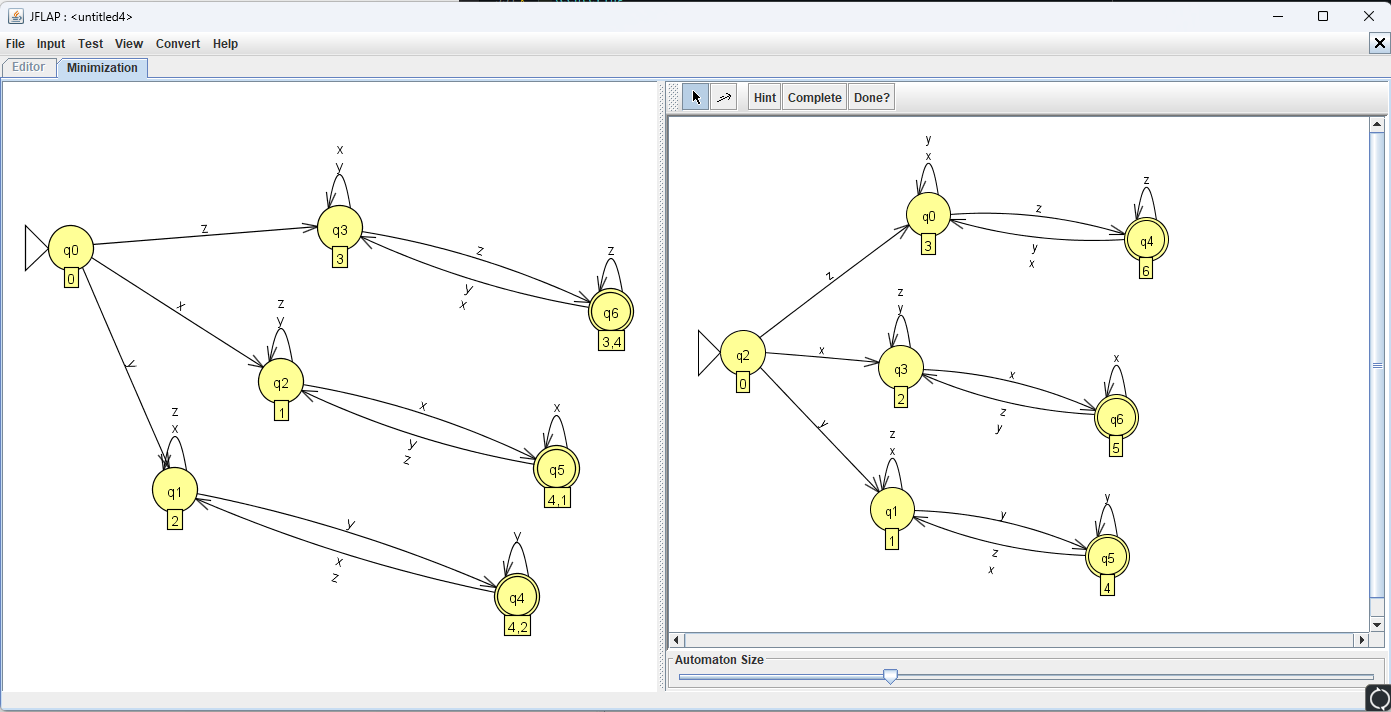
\includegraphics[scale=0.45]{img/DFA_to_DFA_minimized_07.png}
  \caption{DFA mínimo equivalente al NFA}
\end{figure}

\newpage

\chapter{Modificación.}
\section{DFA mínimo sobre el alfabeto $\Sigma = \{0, 1\}$ que reconozca cadenas que no empiezan y terminan por el mismo símbolo o tienen longitud impar.}

\begin{figure}[H]
  \centering
  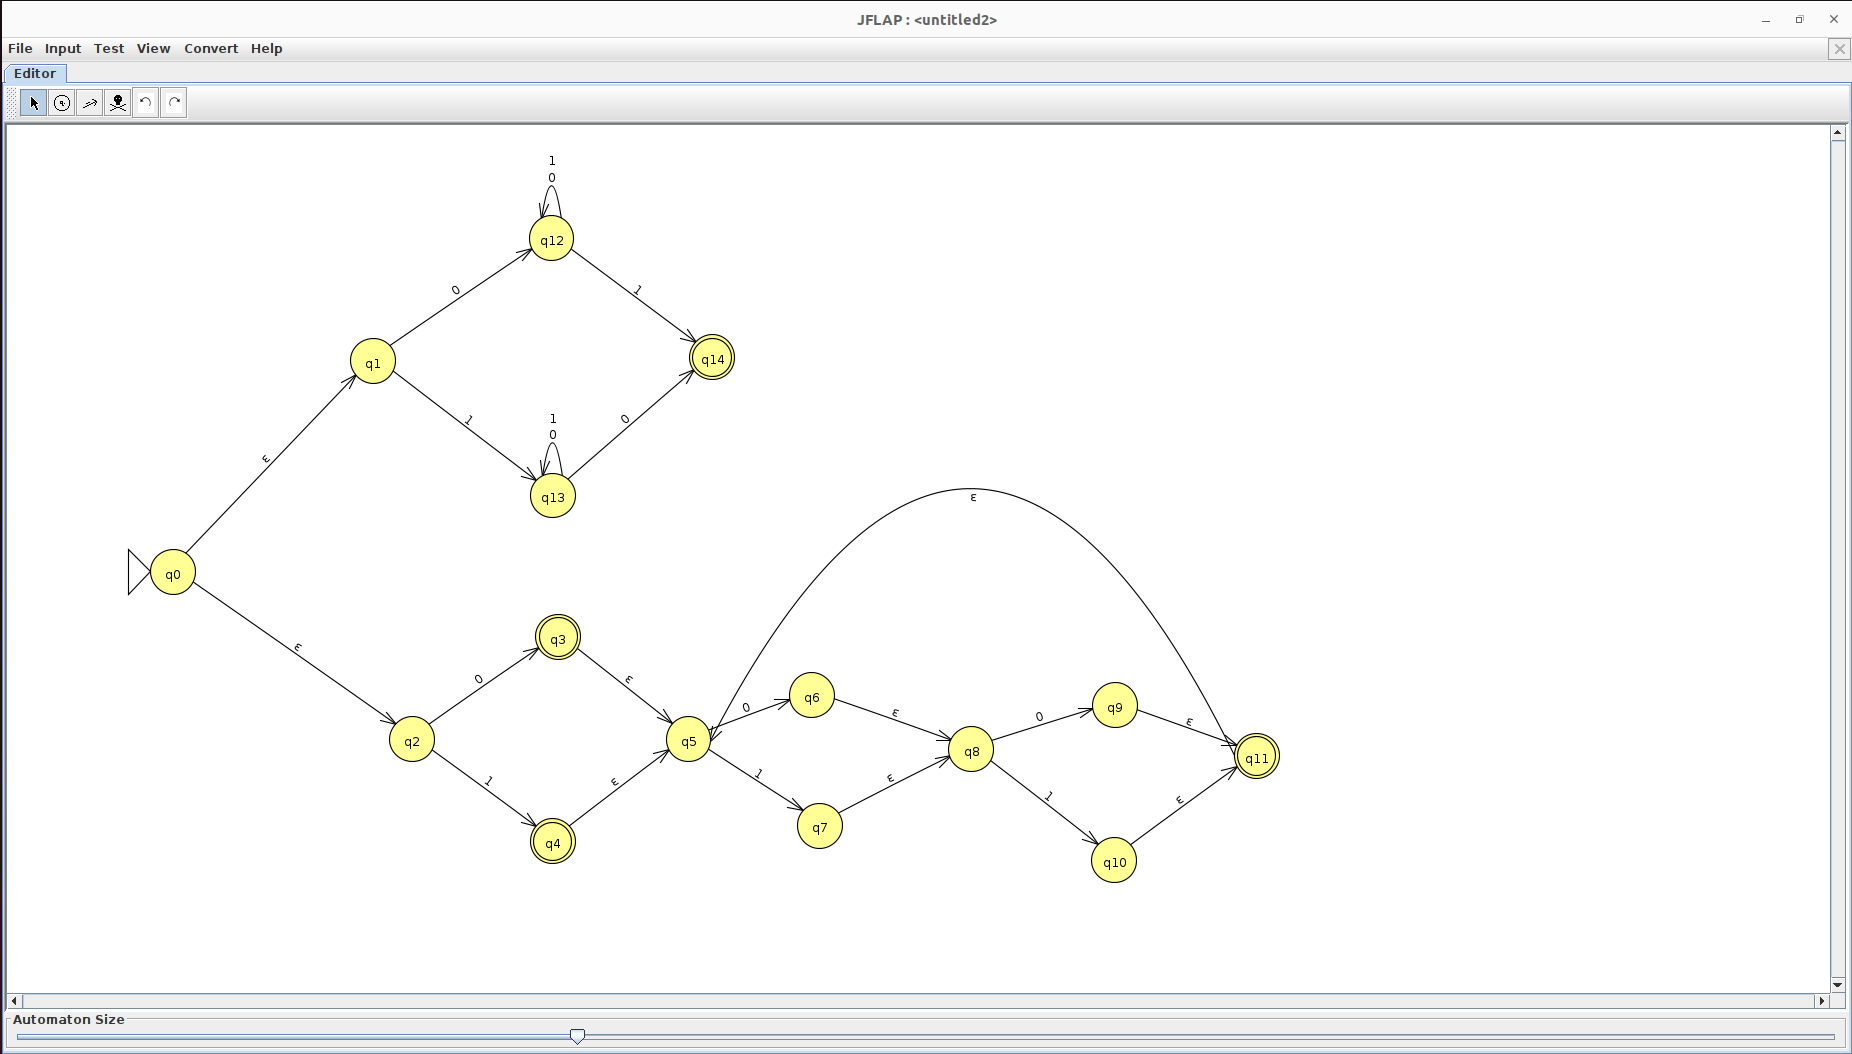
\includegraphics[scale=0.2]{img/nfa_mod.png}
  \caption{NFA Modificación}
\end{figure}

\begin{figure}[H]
  \centering
  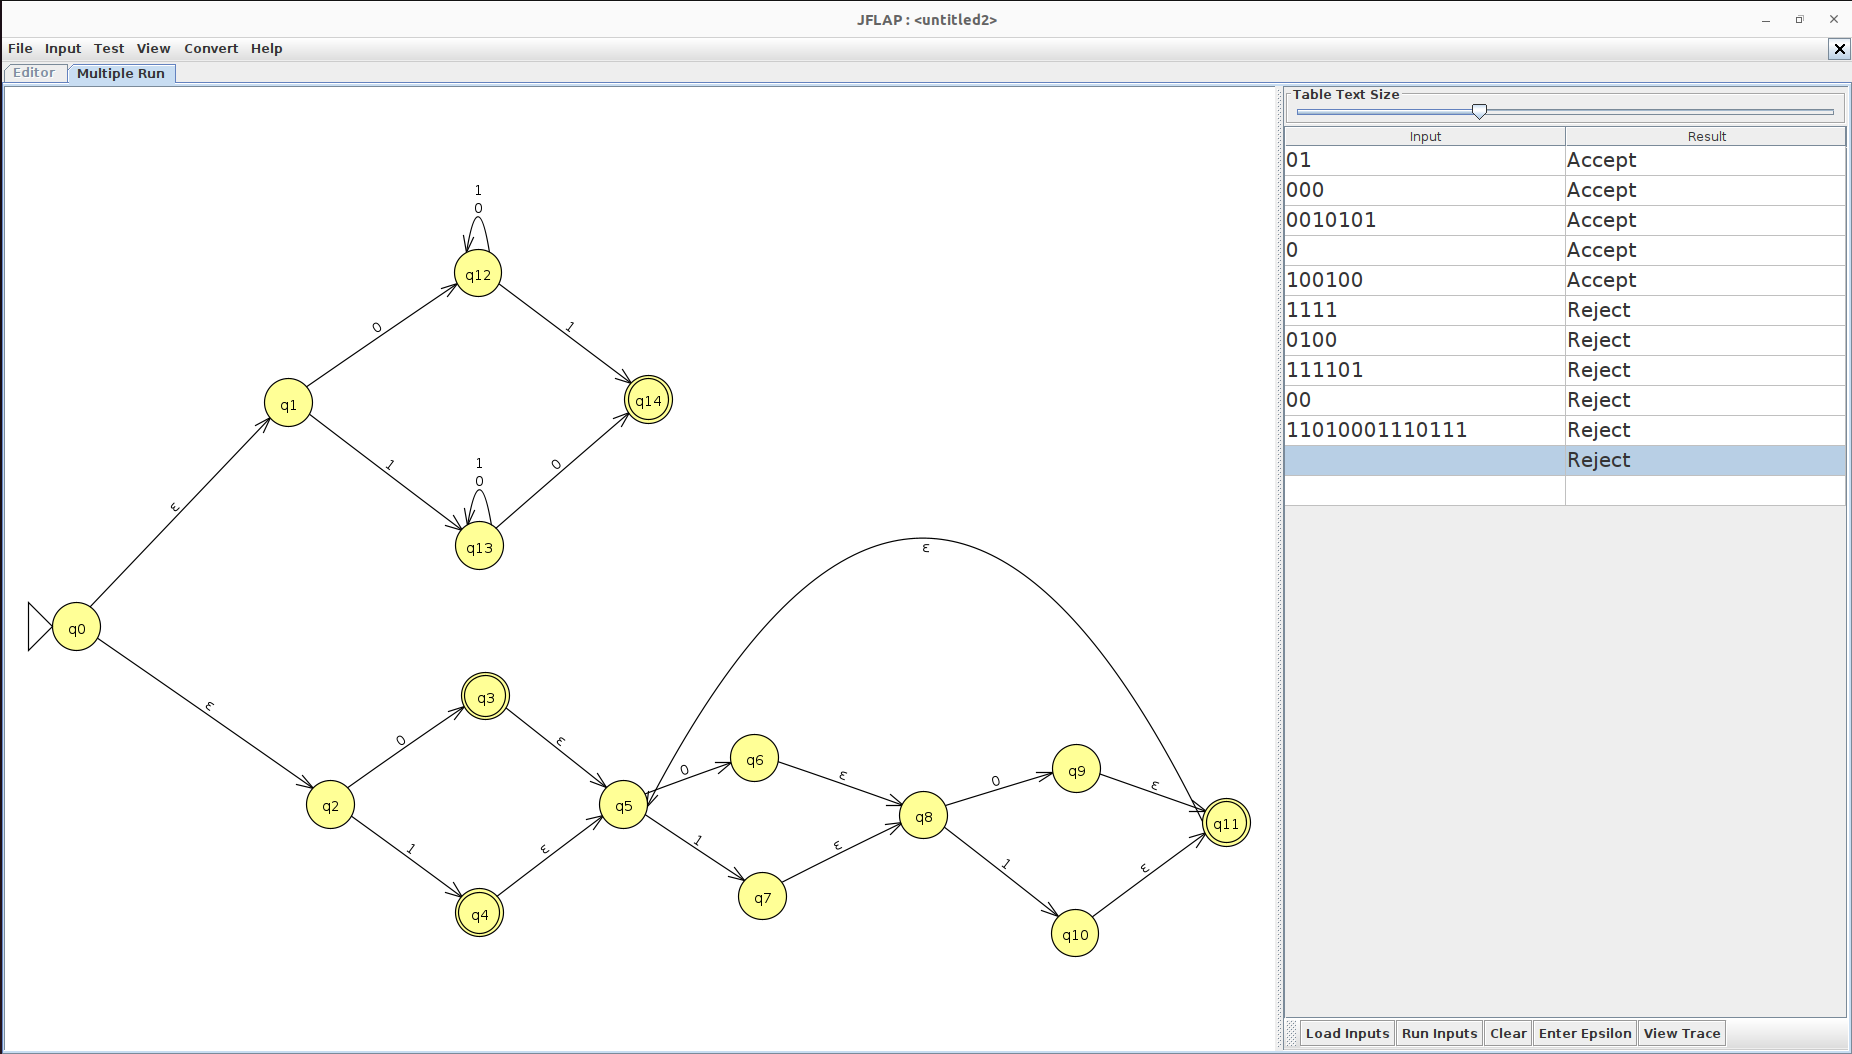
\includegraphics[scale=0.2]{img/Mod_test.png}
  \caption{Cadenas de prueba para el NFA}
\end{figure}

\newpage

Captura de la conversión de NFA a DFA
\begin{figure}[H]
  \centering
  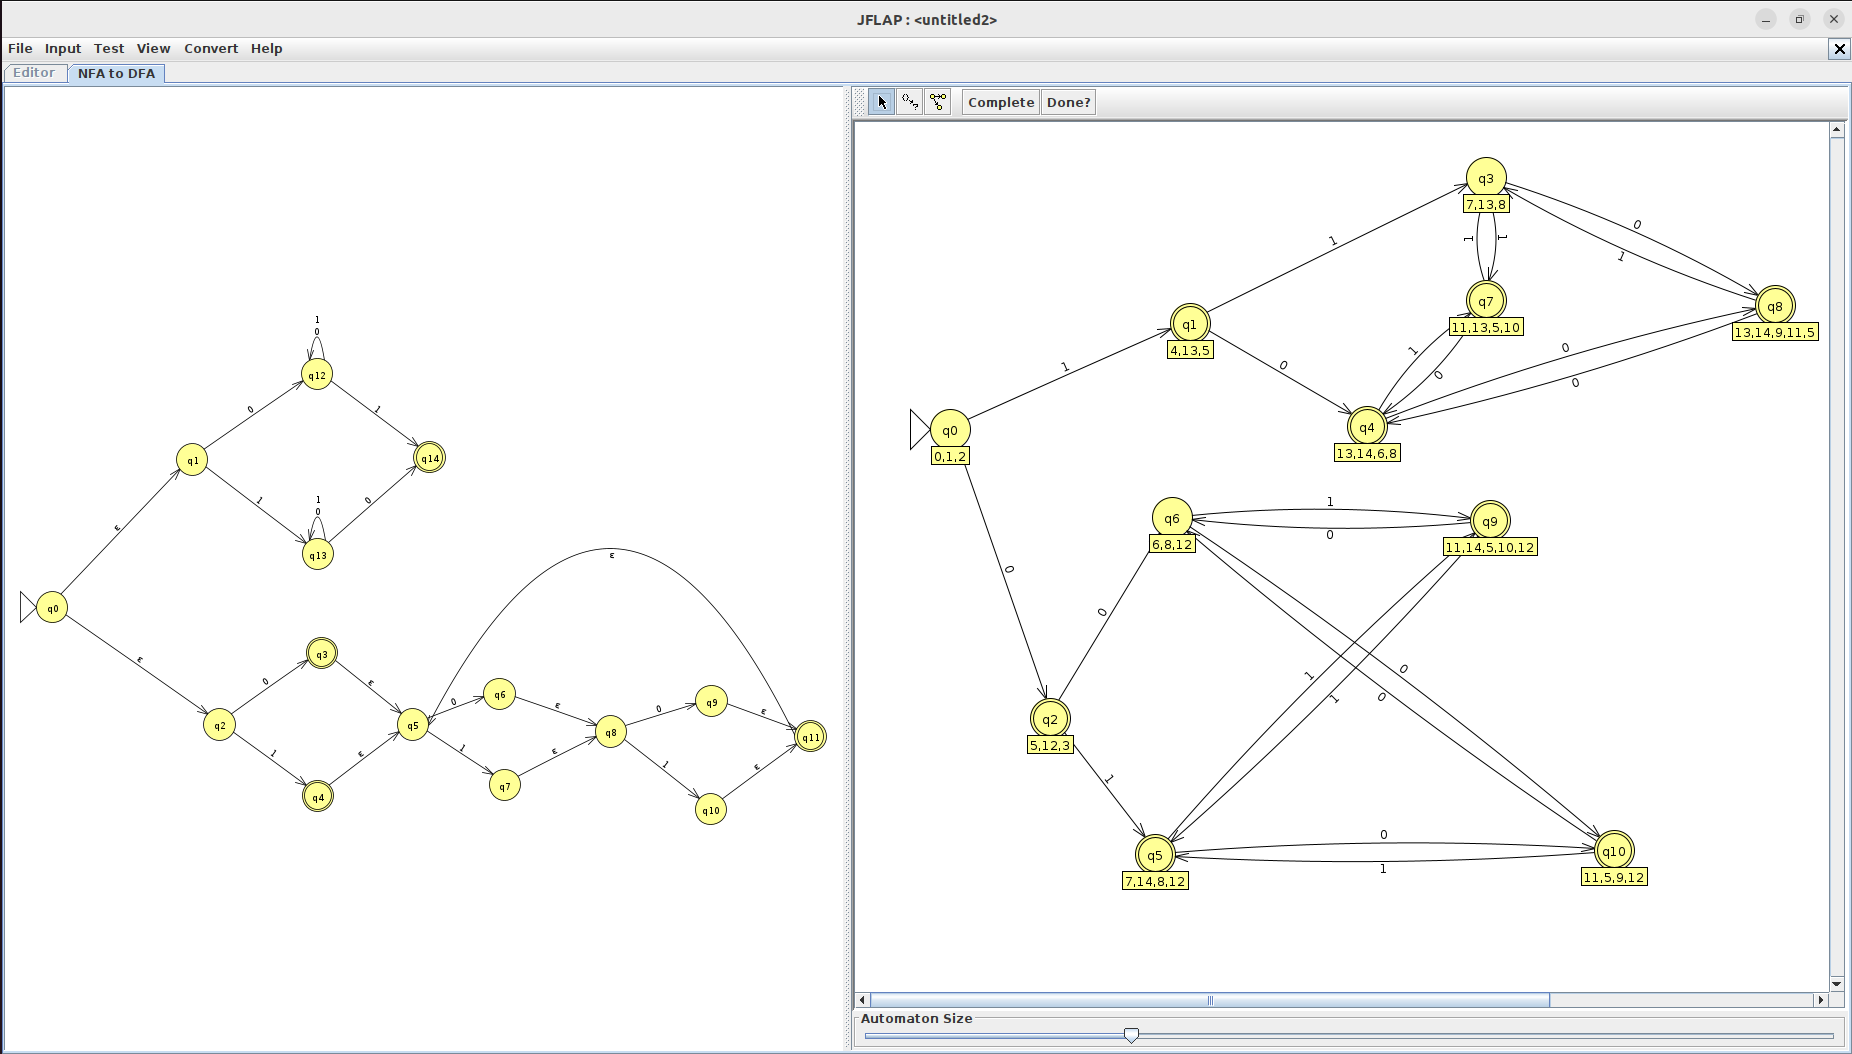
\includegraphics[scale=0.2]{img/mod_nfa_to_dfa.png}
  \caption{NFA a DFA}
\end{figure}

Algoritmo de minimización de DFA
\begin{itemize}
  \item $\{q_1, q_4, q_7, q_8, q_2, q_5, q_9, q_{10}\} \{q_0, q_3, q_6\}$
  \item $\{q_1, q_4, q_7, q_8, q_2, q_5, q_9, q_10\} \{q_0\} \{q_3\} \{q_6\}$
  \item $\{q_1, q_4, q_7, q_8, q_5\} \{q_2, q_9, q_10\} \{q_0\} \{q_3\} \{q_6\}$
  \item $\{q_4, q_5\} \{q_1, q_7, q_8\} \{q_2, q_9, q_10\} \{q_0\} \{q_3\} \{q_6\}$
  \item $\{q_4\} \{q_5\} \{q_1, q_7, q_8\} \{q_2, q_9, q_10\} \{q_0\} \{q_3\} \{q_6\}$
\end{itemize}

\newpage

Resultado de DFA mínimo:
\begin{figure}[H]
  \centering
  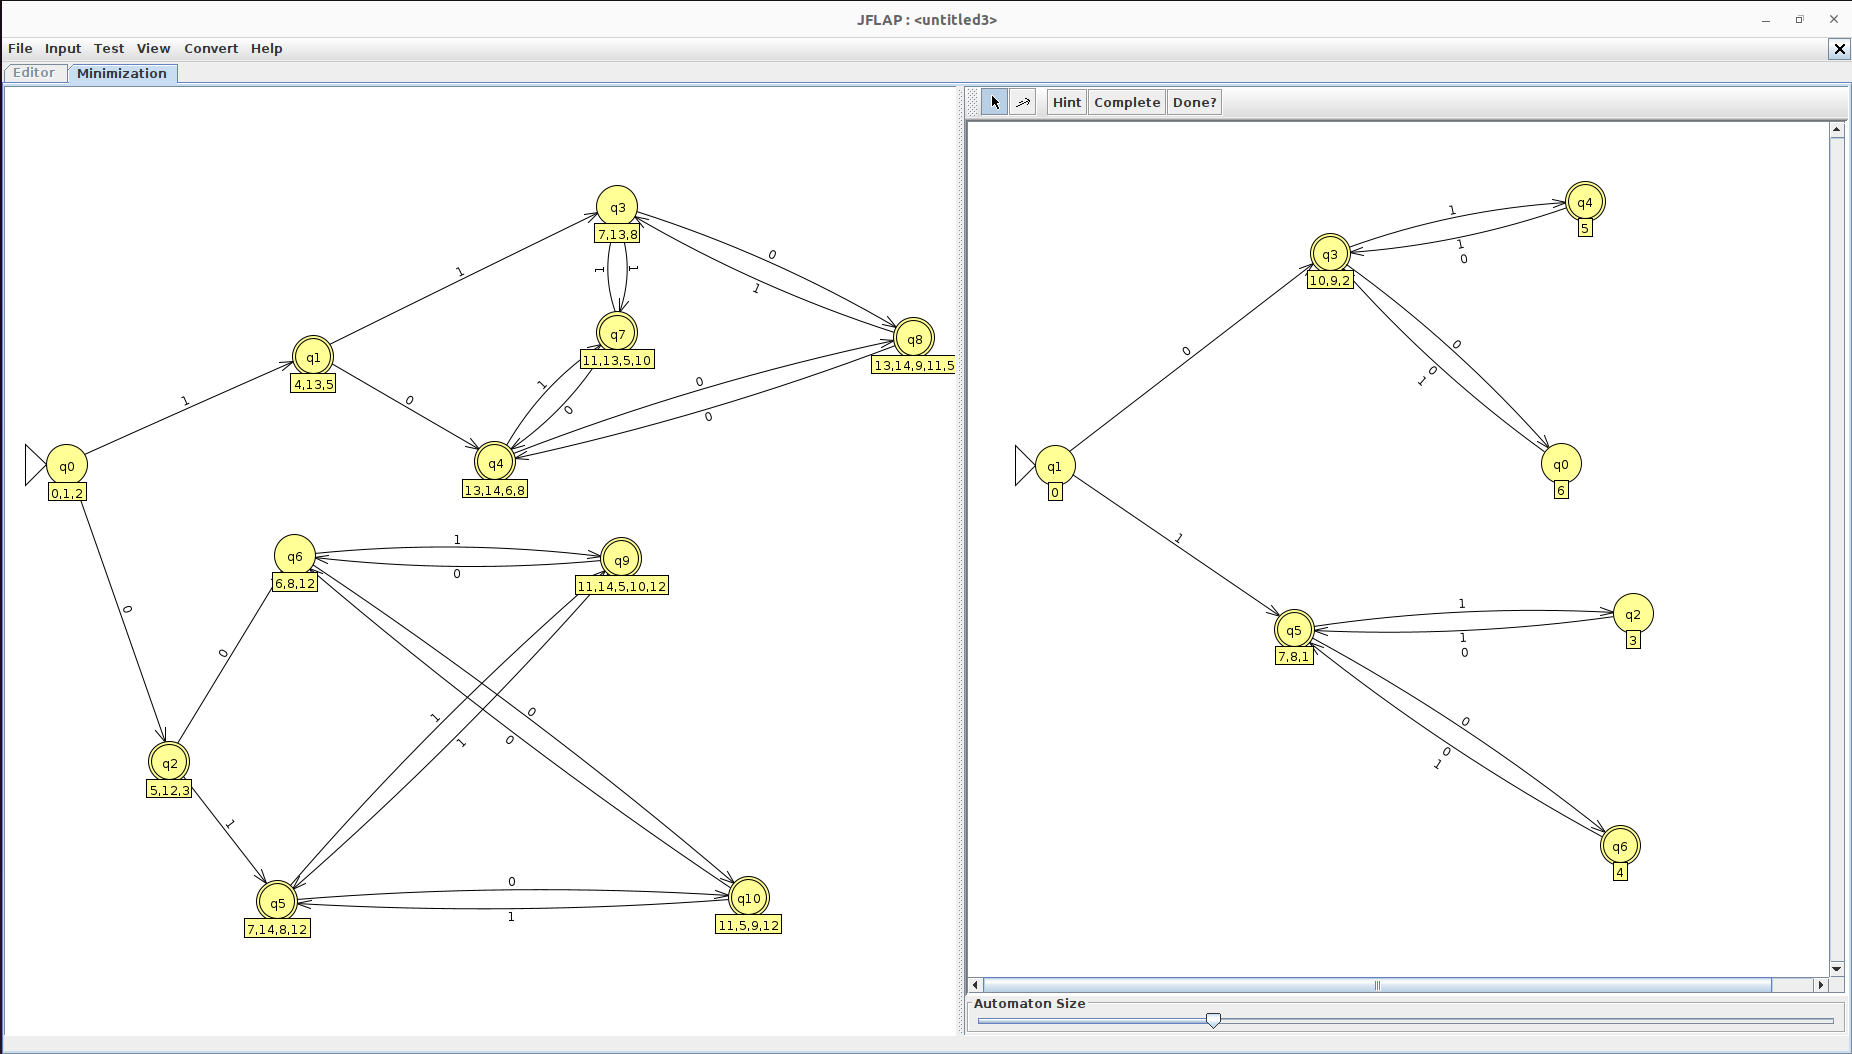
\includegraphics[scale=0.2]{img/mod_minimized.png}
  \caption{DFA mínimo}
\end{figure}

\end{document}